\documentclass[11pt, a4paper]{article}
%\usepackage{proj1}
\usepackage{natbib}
\usepackage{fancyhdr}  
\usepackage{subcaption}
\usepackage{caption}
\usepackage{graphicx}
\usepackage{numprint}
\usepackage{multirow}
\linespread{1.25} 
\setlength{\parindent}{0cm}
\graphicspath{{Images/}}
\usepackage{hyperref}
\usepackage{amsmath}
\usepackage{amsfonts}
\usepackage{amssymb}
\usepackage{amsthm}
\usepackage{mathtools}
\usepackage{commath}
\usepackage{bbm}

%\usepackage[sc,osf]{mathpazo}
\usepackage{subcaption}
\usepackage[a4paper, top=1in, left=1.0in, right=1.0in, bottom=1in, includehead, includefoot]{geometry} %Usually have top as 1in

\usepackage{listings}
\usepackage{color} %red, green, blue, yellow, cyan, magenta, black, white
\definecolor{mygreen}{RGB}{28,172,0} % color values Red, Green, Blue
\definecolor{mylilas}{RGB}{170,55,241}


\hypersetup{colorlinks,linkcolor={black},citecolor={blue},urlcolor={black}}
\usepackage{color}
\urlstyle{same}


\theoremstyle{definition}
\newtheorem{definition}{Definition}[section]

%\newcommand{\Sta}{\rho}
\newcommand{\adja}{q_a}
\newcommand{\adjb}{q_b}
\newcommand{\adjaB}{q_{a,\partial \Omega}}
\newcommand{\adjbB}{q_{b,\partial \Omega}}
%\newcommand{\Con}{u}
\newcommand{\ra}{\rho_a}
\newcommand{\rb}{\rho_b}
\newcommand{\w}{\mathbf{w}}
\newcommand{\Stav}{\mathbf{v}}
\newcommand{\Adja}{\mathbf{p}}
\newcommand{\Adjb}{q}
\newcommand{\Adjc}{{p}_{\partial \Sigma}}
\newcommand{\Con}{\mathbf{f}}
\newcommand{\n}{\mathbf{n}}
\newcommand{\h}{\mathbf{h}}
\newcommand{\K}{\mathbf{K}}


\pagenumbering{gobble}
\begin{document}
	
\section{Optimality conditions for the sedimentation equations}
The relevant part of the equation is:
\begin{align*}
	\nabla \cdot \bigg(\rho \nabla \frac{\delta F[\rho]}{\delta \rho}\bigg)
	&= \frac{1}{\beta} \bigg( \frac{\nabla^2 \rho}{1 - \eta} +  \nabla \rho \cdot \nabla \frac{(3- 2 \eta)}{(1 - \eta)^2}  - \rho \nabla^2\frac{\eta - 2}{(\eta - 1)^2} \bigg),
\end{align*}
where $\eta = a \rho$ and $a = \pi \sigma^2 /4$.
Consider:
\begin{align*}
	F_1(\rho) &= \nabla^2 \rho \frac{1}{1- a\rho}\\
	F_2(\rho) &= \nabla \rho \cdot \nabla \left(\frac{3-2a\rho}{(1-a\rho)^2}\right)\\
	F_3(\rho) &= \rho \nabla^2 \left(\frac{a\rho -2}{(a\rho -1)^2}\right)
\end{align*}
Then
\begin{align*}
	F_1(\rho + h) - F_1(\rho) &= \nabla (\rho +h) \frac{1}{1- a(\rho +h)} - \nabla \rho \frac{1}{1- a\rho}
\end{align*}
Using the expansion: 
\begin{align*}
	\frac{1}{c - x} = \frac{1}{c} + \frac{1}{c^2}x + O(x^2),
\end{align*}
where $c = 1- a \rho$, we get:
\begin{align*}
	F_1(\rho + h) - F_1(\rho) &= \nabla^2 (\rho +h) \left(\frac{1}{1- a\rho} + \frac{a}{(1- a\rho)^2}h \right)- \nabla^2 \rho \frac{1}{1- a\rho}\\
	&= \nabla^2 h \left(\frac{1}{1- a\rho} \right) + \nabla^2 \rho \left(\frac{a}{(1- a\rho)^2}h\right)
\end{align*}
For $F_2$ we consider the expansion:
\begin{align*}
	\frac{1}{(c-x)^2} = \frac{1}{c^2} + \frac{2}{c^3}x + O(x^2),
\end{align*}
and get:
\begin{align*}
	F_2(\rho+h) - F_2(\rho) &= \nabla (\rho +h) \cdot \nabla \left(\frac{3-2a(\rho +h)}{(1-a(\rho+h))^2}\right) -\nabla \rho \cdot \nabla \left(\frac{3-2a\rho}{(1-a\rho)^2}\right) \\
	&= \nabla (\rho +h) \cdot \nabla \left(\frac{3-2a(\rho +h)}{(1-a\rho)^2} + \frac{3-2a(\rho +h)}{(1-a\rho)^3} 2ah \right) -\nabla \rho \cdot \nabla \left(\frac{3-2a\rho}{(1-a\rho)^2}\right)\\
	&=\nabla h \cdot \nabla \left(\frac{3-2a\rho}{(1-a\rho)^2} \right) + \nabla \rho \cdot \nabla \left(h\left(\frac{-2a }{(1-a\rho)^2} + \frac{6a-4a^2  \rho}{(1-a\rho)^3}  \right)\right)\\
	& = \nabla h \cdot \nabla \left( \frac{3-2a\rho}{(1-a\rho)^2} \right) + \left(\nabla h \cdot \nabla \rho \right) \left( \frac{-2a }{(1-a\rho)^2} + \frac{6a-4a^2  \rho}{(1-a\rho)^3}  \right) \\
	&+ h \nabla \rho \cdot \nabla \left(\frac{-2a }{(1-a\rho)^2} + \frac{6a-4a^2  \rho}{(1-a\rho)^3}  \right)
\end{align*}

Finally, we have:
\begin{align*}
	F_3(\rho+h) - F_3(\rho) &= (\rho +h) \nabla^2 \left(\frac{a(\rho +h) -2}{(a(\rho +h) -1)^2}\right) -\rho \nabla^2 \left(\frac{a\rho -2}{(a\rho -1)^2}\right)\\
	&=  (\rho +h) \nabla^2 \left(\frac{a(\rho +h) -2}{(1-a\rho)^2} + \frac{a(\rho +h) -2}{(1-a\rho)^3}2ah \right) -\rho \nabla^2 \left(\frac{a\rho -2}{(a\rho -1)^2}\right)\\
	&= h \nabla^2 \left(\frac{a\rho -2}{(a\rho -1)^2}\right) + \rho \nabla^2  \left(h\left(\frac{a }{(1-a\rho)^2} + \frac{2a^2\rho -4a}{(1-a\rho)^3} \right)\right)\\
	&= h \nabla^2 \left(\frac{a\rho -2}{(a\rho -1)^2}\right) + \rho  \left(\frac{a }{(1-a\rho)^2} + \frac{2a^2\rho -4a}{(1-a\rho)^3} \right)\nabla^2 h \\
	&+ \rho \nabla \left(\frac{a }{(1-a\rho)^2} + \frac{2a^2\rho -4a}{(1-a\rho)^3} \right) \cdot \nabla h + \rho h \nabla^2  \left(\frac{a }{(1-a\rho)^2} + \frac{2a^2\rho -4a}{(1-a\rho)^3} \right)\\
\end{align*}

Combining these in the Lagrangian gives:
\begin{align*}
	\mathcal{L}_\rho(\rho,\w,q)h &= -\frac{1}{\beta}\int_0^T \int_\Omega q \nabla^2 h \left(\frac{1}{1- a\rho} \right) + q\nabla^2 \rho \left(\frac{a}{(1- a\rho)^2}h\right)\\
	&+ q\nabla h \cdot \nabla \left( \frac{3-2a\rho}{(1-a\rho)^2} \right) + q\left(\nabla h \cdot \nabla \rho \right) \left( \frac{-2a }{(1-a\rho)^2} + \frac{6a-4a^2  \rho}{(1-a\rho)^3}  \right) \\
	&+ qh \nabla \rho \cdot \nabla \left(\frac{-2a }{(1-a\rho)^2} + \frac{6a-4a^2  \rho}{(1-a\rho)^3}  \right)\\
	&- qh \nabla^2 \left(\frac{a\rho -2}{(a\rho -1)^2}\right) - q\rho  \left(\frac{a }{(1-a\rho)^2} + \frac{2a^2\rho -4a}{(1-a\rho)^3} \right)\nabla^2 h \\
	&- q\rho \nabla \left(\frac{a }{(1-a\rho)^2} + \frac{2a^2\rho -4a}{(1-a\rho)^3} \right) \cdot \nabla h - q\rho h \nabla^2  \left(\frac{a }{(1-a\rho)^2} + \frac{2a^2\rho -4a}{(1-a\rho)^3} \right).
\end{align*}
Rearranging gives:
\begin{align*}
	\mathcal{L}_\rho(\rho,\w,q)h &= -\frac{1}{\beta}\int_0^T \int_\Omega h \bigg(q\nabla^2 \rho \left(\frac{a}{(1- a\rho)^2}\right)  + q \nabla \rho \cdot \nabla \left(\frac{-2a }{(1-a\rho)^2} \right) - q \nabla^2 \left(\frac{a\rho -2}{(a\rho -1)^2}\right)\\
	&- q\rho  \nabla^2  \left(\frac{a }{(1-a\rho)^2} + \frac{2a^2\rho -4a}{(1-a\rho)^3} \right)\bigg)\\
	&+ \nabla h \cdot \bigg( q  \nabla \left( \frac{3-2a\rho}{(1-a\rho)^2} \right) + q \nabla \rho  \left( \frac{-2a }{(1-a\rho)^2} + \frac{6a-4a^2  \rho}{(1-a\rho)^3}  \right)- q\rho \nabla \left(\frac{a }{(1-a\rho)^2} + \frac{2a^2\rho -4a}{(1-a\rho)^3} \right) \bigg)\\
	&+ \nabla^2 h \bigg(q \left(\frac{1}{1- a\rho} \right)  - q\rho  \left(\frac{a }{(1-a\rho)^2} + \frac{2a^2\rho -4a}{(1-a\rho)^3} \right)  \bigg)
\end{align*}
Integration by parts gives:
\begin{align*}
	\mathcal{L}_\rho(\rho,\w,q)h &= -\frac{1}{\beta}\int_0^T \int_\Omega h \bigg(q\nabla^2 \rho \left(\frac{a}{(1- a\rho)^2}\right)  + q \nabla \rho \cdot \nabla \left(\frac{-2a }{(1-a\rho)^2} \right) - q \nabla^2 \left(\frac{a\rho -2}{(a\rho -1)^2}\right)\\
	&- q\rho  \nabla^2  \left(\frac{a }{(1-a\rho)^2} + \frac{2a^2\rho -4a}{(1-a\rho)^3} \right)\bigg)\\
	&-  h \nabla \bigg( q  \nabla \left( \frac{3-2a\rho}{(1-a\rho)^2} \right) + q \nabla \rho  \left( \frac{-2a }{(1-a\rho)^2} + \frac{6a-4a^2  \rho}{(1-a\rho)^3}  \right)- q\rho \nabla \left(\frac{a }{(1-a\rho)^2} + \frac{2a^2\rho -4a}{(1-a\rho)^3} \right) \bigg)\\
	&+  h \nabla^2\bigg(q \left(\frac{1}{1- a\rho} \right)  - q\rho  \left(\frac{a }{(1-a\rho)^2} + \frac{2a^2\rho -4a}{(1-a\rho)^3} \right)  \bigg)
\end{align*}
So we have:
\begin{align*}
	\mathcal{L}_\rho(\rho,\w,q)h &= -\frac{1}{\beta}\int_0^T\int_\Omega h \bigg[  q\nabla^2 \rho \left(\frac{a}{(1- a\rho)^2}\right)  + q \nabla \rho \cdot \nabla \left(\frac{-2a }{(1-a\rho)^2} \right) - q \nabla^2 \left(\frac{a\rho -2}{(a\rho -1)^2}\right)\\
	&- q\rho  \nabla^2  \left(\frac{a }{(1-a\rho)^2} \right) - q\rho  \nabla^2  \left(\frac{2a^2\rho -4a}{(1-a\rho)^3} \right)\\
	& -\nabla \cdot \left( q  \nabla \left( \frac{3-2a\rho}{(1-a\rho)^2} \right) \right) - \nabla \cdot \left( q \nabla \rho  \left( \frac{-2a }{(1-a\rho)^2} \right)\right)  - \nabla \cdot \left( q \nabla \rho  \left(\frac{6a-4a^2  \rho}{(1-a\rho)^3}  \right)\right)  \\
	& + \nabla \cdot\left( q\rho \nabla \left(\frac{a }{(1-a\rho)^2} \right) \right) + \nabla \cdot\left( q\rho \nabla \left( \frac{2a^2\rho -4a}{(1-a\rho)^3} \right) \right)\\
	&+   \nabla^2 \left(q \left(\frac{1}{1- a\rho} \right) \right) - \nabla^2 \left(q\rho  \left(\frac{a }{(1-a\rho)^2}\right)\right) - \nabla^2 \left(q\rho \left(\frac{2a^2\rho -4a}{(1-a\rho)^3} \right)\right)\bigg] dr dt 
\end{align*}

\subsection{Boundary Terms}
We have the equation:
\begin{align*}
	\rho \nabla \frac{\delta F[\rho]}{\delta \rho} &= \frac{1}{\beta} \bigg(  \frac{\nabla \rho}{1 - \eta}  - \rho \nabla\frac{\eta - 2}{(\eta - 1)^2}  \bigg)
\end{align*}
Then:
\begin{align*}
	F_4(\rho) &= \frac{\nabla \rho}{1 - a \rho}\\
	F_5(\rho) &= \rho \nabla\frac{a \rho - 2}{(a \rho - 1)^2}  
\end{align*}
Then for $F_4$ we have:
\begin{align*}
	F_4(\rho+h) - F_4(\rho) &=\nabla (\rho + h) \frac{1}{1 - a (\rho + h)} - \nabla \rho \frac{1}{1 - a \rho}\\
	&= \nabla(\rho + h) \left(\frac{1}{1 - a\rho} + \frac{1}{(1 -a \rho)^2}h \right)\\
	&= \nabla h \left(\frac{1}{1 - a\rho}\right) + \nabla \rho \left( \frac{1}{(1 -a \rho)^2}h \right)
\end{align*}
For $F_5$ we get:
\begin{align*}
	F_5(\rho + h) - F_5(\rho) &= (\rho + h) \nabla\frac{a (\rho +h) - 2}{(a (\rho +h) - 1)^2}  - \rho \nabla\frac{a \rho - 2}{(a \rho - 1)^2} \\
	&=(\rho + h) \nabla \left( \frac{a (\rho +h) - 2}{(1- a \rho)^2} + \frac{a (\rho +h) - 2}{(1- a \rho)^3} 2ah\right) - \rho \nabla\frac{a \rho - 2}{(a \rho - 1)^2} \\
	&= h \nabla \left(\frac{a \rho  - 2}{(1- a \rho)^2}\right) + \rho \nabla \left( h\left( \frac{a}{(1- a \rho)^2} + \frac{2a^2\rho - 4a}{(1- a \rho)^3} \right)\right)\\
	&= h \nabla \left(\frac{a \rho  - 2}{(1- a \rho)^2}\right) + h \rho \nabla \left( \frac{a}{(1- a \rho)^2} + \frac{2a^2\rho - 4a}{(1- a \rho)^3} \right) + \nabla h \left( \rho \frac{a}{(1- a \rho)^2} + \rho\frac{2a^2\rho - 4a}{(1- a \rho)^3} \right)
\end{align*}

Then the boundary terms for the Lagrangian are:
\begin{align*}
	\mathcal{L}_{\rho,1}(\rho,\w, q) h &= - \frac{1}{\beta}\int_0^T \int_{\partial \Omega} \bigg( q_{\partial \Omega}\nabla h \left(\frac{1}{1 - a\rho}\right) + q_{\partial \Omega}\nabla \rho \left( \frac{1}{(1 -a \rho)^2}h \right)- q_{\partial \Omega}h \nabla \left(\frac{a \rho  - 2}{(1- a \rho)^2}\right) \\
	&- h q_{\partial \Omega}\rho \nabla \left( \frac{a}{(1- a \rho)^2} + \frac{2a^2\rho - 4a}{(1- a \rho)^3} \right) - q_{\partial \Omega}\nabla h \left( \rho \frac{a}{(1- a \rho)^2} + \rho\frac{2a^2\rho - 4a}{(1- a \rho)^3} \right) \bigg) \cdot \n dr dt
\end{align*}

From the integration by parts of the terms within the domain we get:
\begin{align*}
	\mathcal{L}_{\rho,2}(\rho, \w,q)h &= - \frac{1}{\beta}\int_0^T \int_{\partial \Omega} \bigg(h \bigg( q  \nabla \left( \frac{3-2a\rho}{(1-a\rho)^2} \right) + q \nabla \rho  \left( \frac{-2a }{(1-a\rho)^2} + \frac{6a-4a^2  \rho}{(1-a\rho)^3}  \right)\\
	&- q\rho \nabla \left(\frac{a }{(1-a\rho)^2} + \frac{2a^2\rho -4a}{(1-a\rho)^3} \right) \bigg)\\
	& + \nabla h \bigg(q \left(\frac{1}{1- a\rho} \right)  - q\rho  \left(\frac{a }{(1-a\rho)^2} + \frac{2a^2\rho -4a}{(1-a\rho)^3} \right)  \bigg) \\
	&- h \nabla \bigg(q \left(\frac{1}{1- a\rho} \right)  - q\rho  \left(\frac{a }{(1-a\rho)^2} + \frac{2a^2\rho -4a}{(1-a\rho)^3} \right)  \bigg) \bigg)\cdot \n dr dt
\end{align*}


Combining all of these give all boundary terms for the Lagrangian:
\begin{align*}
	\mathcal{L}_\rho (\rho,\w,q)h &= - \frac{1}{\beta}\int_0^T \int_{\partial \Omega} \bigg( h \bigg(  q_{\partial \Omega}\nabla \rho \left( \frac{1}{(1 -a \rho)^2} \right)- q_{\partial \Omega} \nabla \left(\frac{a \rho  - 2}{(1- a \rho)^2}\right) \\
	&-  q_{\partial \Omega}\rho \nabla \left( \frac{a}{(1- a \rho)^2} + \frac{2a^2\rho - 4a}{(1- a \rho)^3} \right)
	+ \bigg( q  \nabla \left( \frac{3-2a\rho}{(1-a\rho)^2} \right) + q \nabla \rho  \left( \frac{-2a }{(1-a\rho)^2} + \frac{6a-4a^2  \rho}{(1-a\rho)^3}  \right)\\
	&- q\rho \nabla \left(\frac{a }{(1-a\rho)^2} + \frac{2a^2\rho -4a}{(1-a\rho)^3} \right) \bigg) -  \nabla \bigg(q \left(\frac{1}{1- a\rho} \right)  - q\rho  \left(\frac{a }{(1-a\rho)^2} + \frac{2a^2\rho -4a}{(1-a\rho)^3} \right)  \bigg)	\bigg)\\
	& +\nabla h \bigg( q_{\partial \Omega} \left(\frac{1}{1 - a\rho}\right) - q_{\partial \Omega}\left( \rho \frac{a}{(1- a \rho)^2} + \rho\frac{2a^2\rho - 4a}{(1- a \rho)^3} \right) +q \left(\frac{1}{1- a\rho} \right) \\
	& - q\rho  \left(\frac{a }{(1-a\rho)^2} + \frac{2a^2\rho -4a}{(1-a\rho)^3} \right)  \bigg) \bigg) \cdot \n dr dt
\end{align*}
Comparing terms in $\nabla h$ (there should be $\cdot \n$ everywhere in the below):
\begin{align*}
	&q_{\partial \Omega} \left(\frac{1}{1 - a\rho}\right) - q_{\partial \Omega}\left( \rho \frac{a}{(1- a \rho)^2} + \rho\frac{2a^2\rho - 4a}{(1- a \rho)^3} \right) \\
	&+q \left(\frac{1}{1- a\rho} \right)  - q\rho  \left(\frac{a }{(1-a\rho)^2} + \frac{2a^2\rho -4a}{(1-a\rho)^3} \right)  = 0.
\end{align*}
This holds when $q_{\partial \Omega} = -q$.
Then for $h \neq 0$ we get:
\begin{align*}
	&-q\nabla \rho \left( \frac{1}{(1 -a \rho)^2} \right)+q \nabla \left(\frac{a \rho  - 2}{(1- a \rho)^2}\right) \\
	&+q\rho \nabla \left( \frac{a}{(1- a \rho)^2} + \frac{2a^2\rho - 4a}{(1- a \rho)^3} \right)
	+  q  \nabla \left( \frac{3-2a\rho}{(1-a\rho)^2} \right) + q \nabla \rho  \left( \frac{-2a }{(1-a\rho)^2} + \frac{6a-4a^2  \rho}{(1-a\rho)^3}  \right)\\
	&- q\rho \nabla \left(\frac{a }{(1-a\rho)^2} + \frac{2a^2\rho -4a}{(1-a\rho)^3} \right) -  \nabla \bigg(q \left(\frac{1}{1- a\rho} \right)  - q\rho  \left(\frac{a }{(1-a\rho)^2} + \frac{2a^2\rho -4a}{(1-a\rho)^3} \right) \bigg) = 0
\end{align*}
Then:
\begin{align*}
	&q \bigg( \nabla \left(\frac{a \rho  - 2}{(1- a \rho)^2} + \frac{3-2a\rho}{(1-a\rho)^2} \right) + \nabla \rho  \left( \frac{-2a }{(1-a\rho)^2} - \frac{1}{(1 -a \rho)^2} + \frac{6a-4a^2  \rho}{(1-a\rho)^3}  \right)\bigg)\\
	& -  \nabla \bigg(q \left(\frac{1}{1- a\rho} \right)  - q\rho  \left(\frac{a }{(1-a\rho)^2} + \frac{2a^2\rho -4a}{(1-a\rho)^3} \right) \bigg) = 0	
\end{align*}
and so:
\begin{align*}
	&q \bigg( \nabla \left(\frac{a \rho  - 2}{(1- a \rho)^2} + \frac{3-2a\rho}{(1-a\rho)^2} \right) + \nabla \rho  \left( \frac{-2a }{(1-a\rho)^2} - \frac{1}{(1 -a \rho)^2} + \frac{6a-4a^2  \rho}{(1-a\rho)^3}  \right)\bigg)\\
	& + q \nabla \bigg( \left(\frac{1}{1- a\rho} \right)  - \rho  \left(\frac{a }{(1-a\rho)^2} + \frac{2a^2\rho -4a}{(1-a\rho)^3} \right) \bigg) -  \nabla q\bigg( \left(\frac{1}{1- a\rho} \right)  - \rho  \left(\frac{a }{(1-a\rho)^2} + \frac{2a^2\rho -4a}{(1-a\rho)^3} \right) \bigg)  = 0	\\
\end{align*}
The terms with $\nabla q$ don't cancel nicely so there is a mistake somewhere.
\begin{align*}
	&q \bigg( \nabla \left(\frac{-2a \rho  +1}{(1- a \rho)^2} \right) + \nabla \rho  \left( \frac{-2a }{(1-a\rho)^2} - \frac{1}{(1 -a \rho)^2} + \frac{6a-4a^2  \rho}{(1-a\rho)^3}  \right) +\nabla \bigg( \left(\frac{1}{1- a\rho} \right)  - \rho  \left( \frac{2a^2\rho -4a}{(1-a\rho)^3} \right) \bigg) \bigg)\\
	&-  \nabla q\bigg( \left(\frac{1}{1- a\rho} \right)  - \rho  \left(\frac{a }{(1-a\rho)^2} + \frac{2a^2\rho -4a}{(1-a\rho)^3} \right) \bigg)  = 0	\\
\end{align*}
	
	\section{Flow through constriction}
	First Question: Why are the stripes there. If we look at $V_{ext}$ in one dimension, no oscillation is noticeable, see Figure \ref{F1a} and Figure \ref{F2a} and \ref{F3a}.\\
	\\
	Second Question: How to improve the performance with the transformation. We have $\rho = \exp(h -V_{ext})$. The issue was that $\rho$ is zero at some point so $h = \ln \rho + V_{ext}$ was the point of trouble, since we get points at negative infinity. I added $10^{-5}$ to $\rho_0$ to circumvent that but it's still very slow and I am not sure if it's doing much better than the non-transformed problem.  In fact, it runs to the end but gives a warning that the integration tolerances cannot be met, so it looks like it's worse than the original. And it even struggles with the case without the constriction. I use $n = 30$ and $N =50$ and the initial condition is $\rho = \exp(-V_{ext})$.
	\begin{figure}[h]
		\centering
		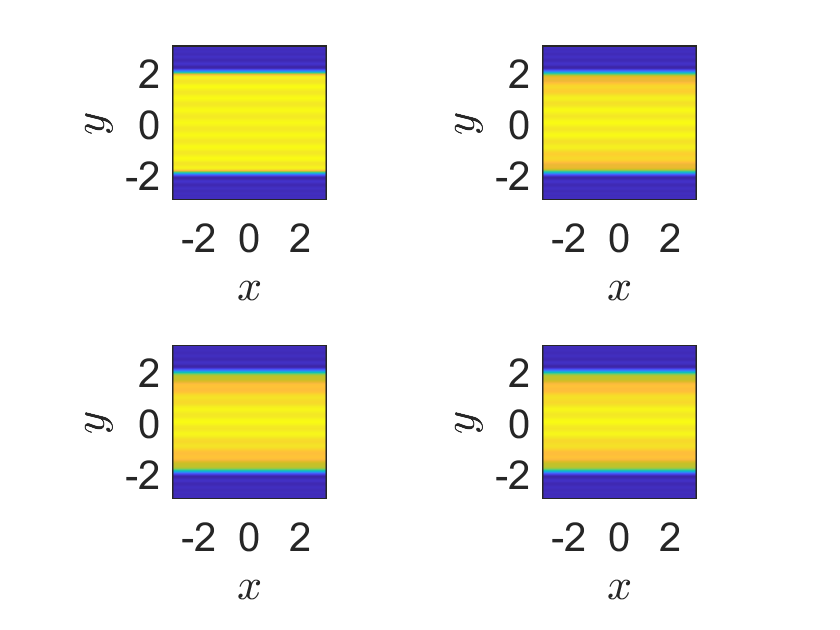
\includegraphics[scale=0.7]{rhoT.png}
		\caption{Stripes in $\rho$ but no oscillation in $V_{ext}$} 
		\label{F3a}
	\end{figure} 
	\begin{figure}[h]
		\centering
		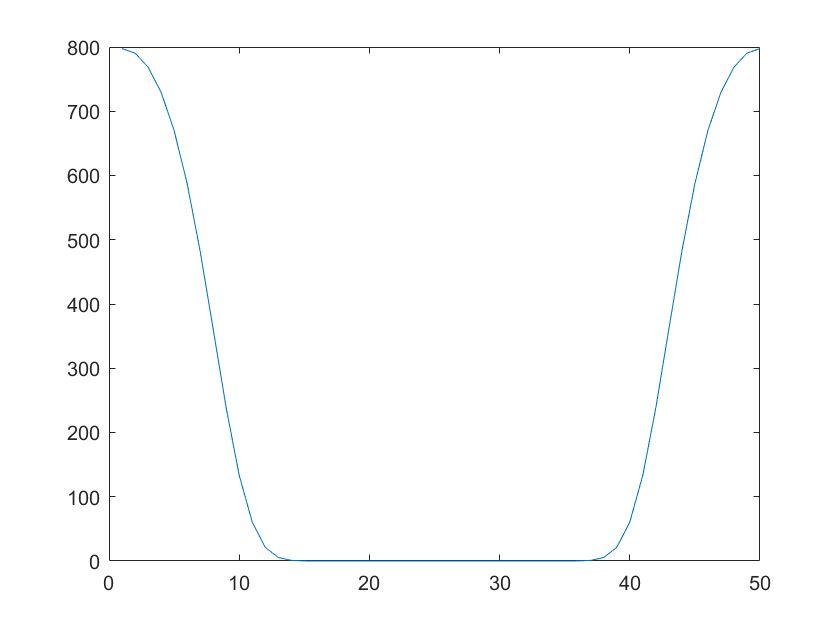
\includegraphics[scale=0.25]{Vext1.png}
		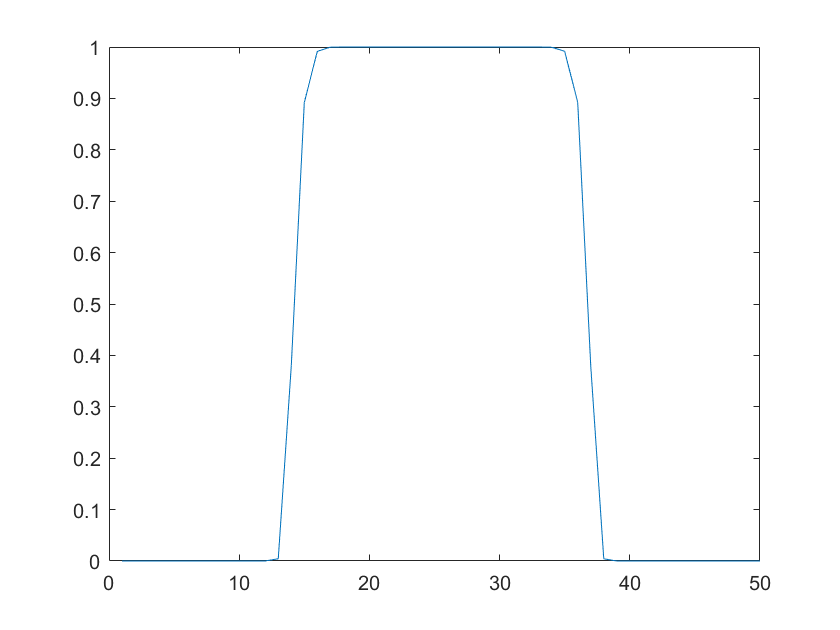
\includegraphics[scale=0.25]{rho1.png}
		\caption{$V_{ext}$ and $\rho$ in 1D, $b =1$} 
		\label{F1a}
	\end{figure} 

	\begin{figure}[h]
		\centering
		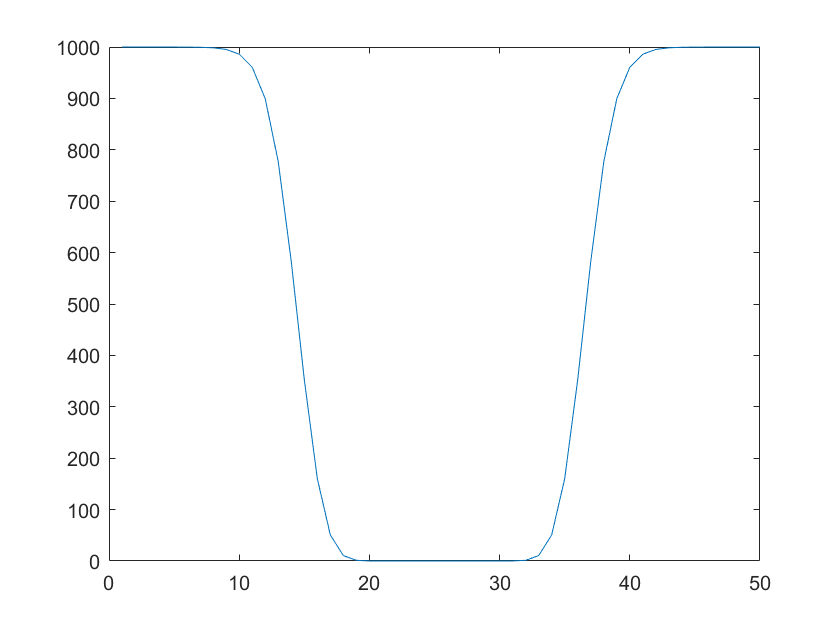
\includegraphics[scale=0.25]{Vext2.png}
		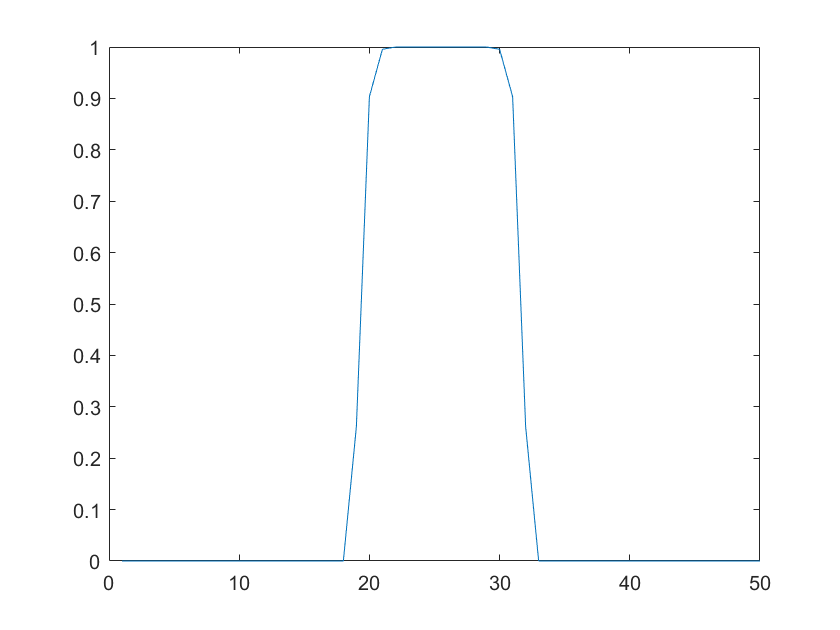
\includegraphics[scale=0.25]{rho2.png}
		\caption{$V_{ext}$ and $\rho$ in 1D, $b =0.7$} 
		\label{F2a}
	\end{figure} 
	
	
	
	\section{Sedimentation Periodic}
	Now that the periodic case is working, I do not know why we do not get the same behaviour as in Archer's paper.
	We are choosing the two configurations in Archer's paper. $\bar \rho = 0.072/\sigma^2$ and $\bar \rho = 0.2 / \sigma^2$. We set the domain to be $43 \times 60$, as in Archer's paper. We use $N = 50$ and $n = 30$, and $TMax = 60$.
	
	At first we consider $\sigma = 1$ and so $\bar \rho = 0.072$, see Figure \ref{F4}. 
	\begin{figure}[h]
		\centering
		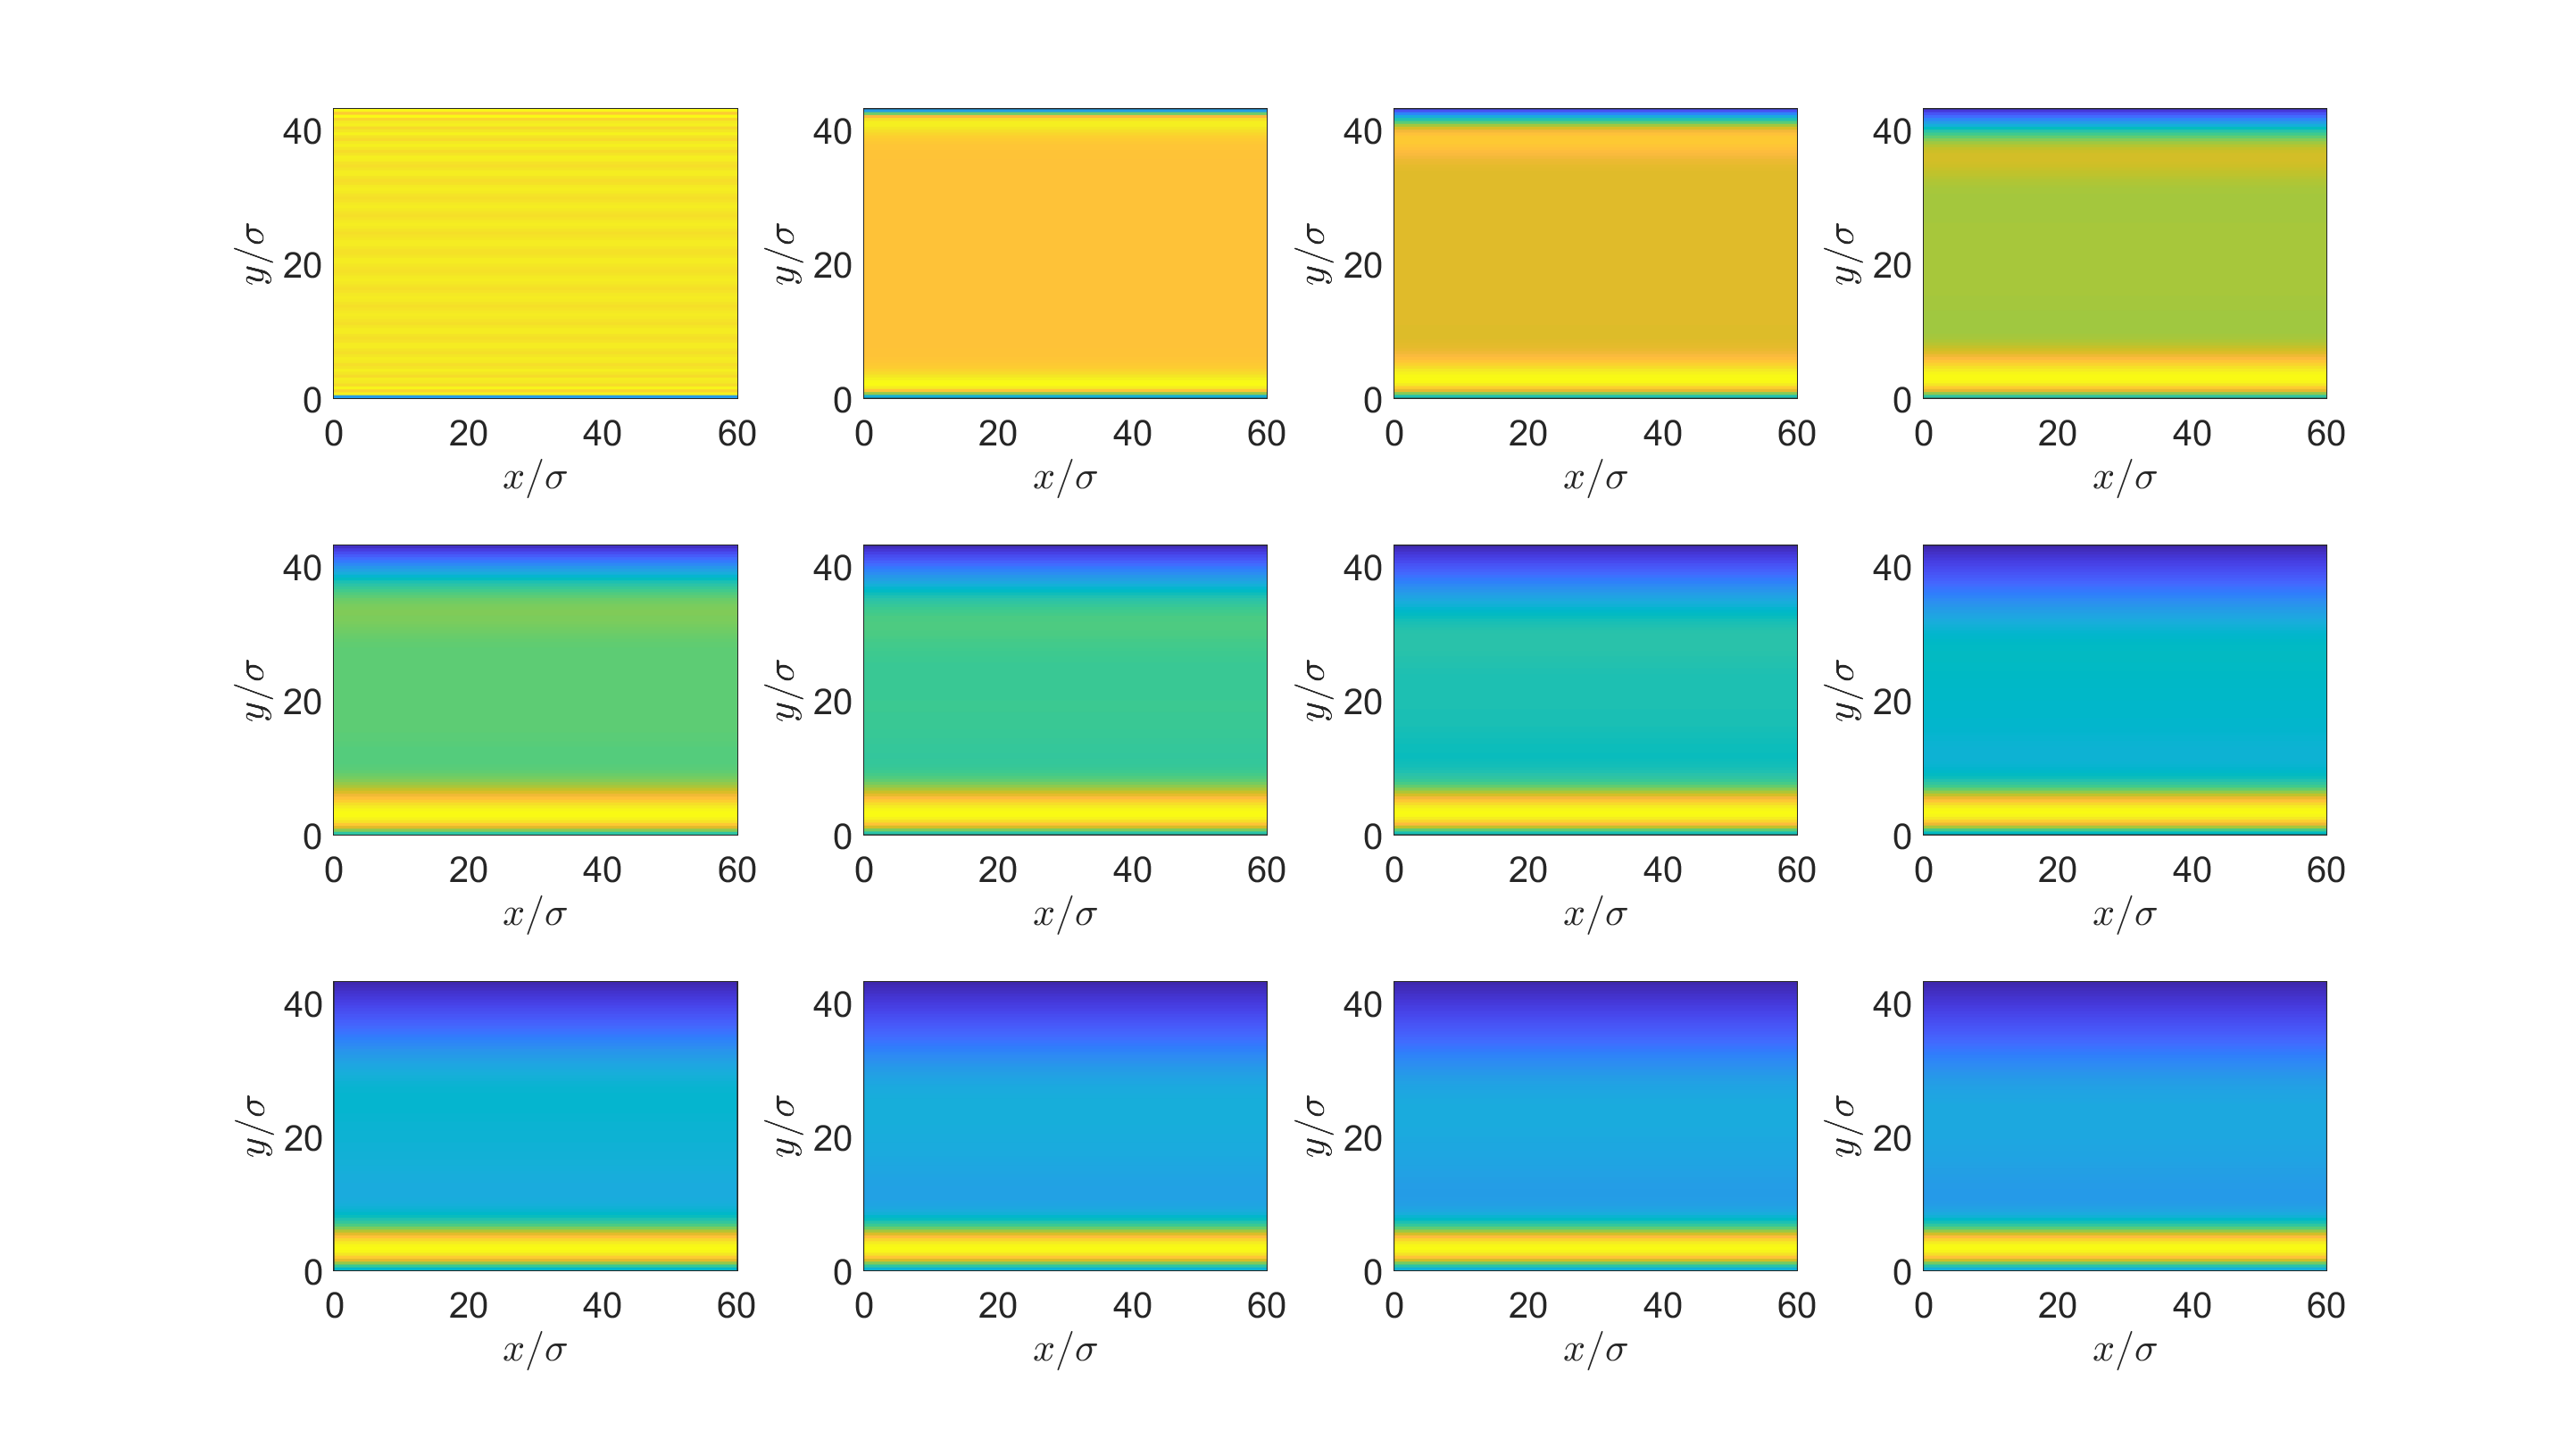
\includegraphics[scale=0.25]{Periodic1.png}
		\caption{$\sigma =1$, $\bar \rho =0.072$} 
		\label{F4}
	\end{figure}
	Then we consider $\sigma = 0.5$ and so $\bar \rho = 0.072$, see Figure \ref{F5}. We get a similar behaviour, but the times are not quite the same.
	\begin{figure}[h]
		\centering
		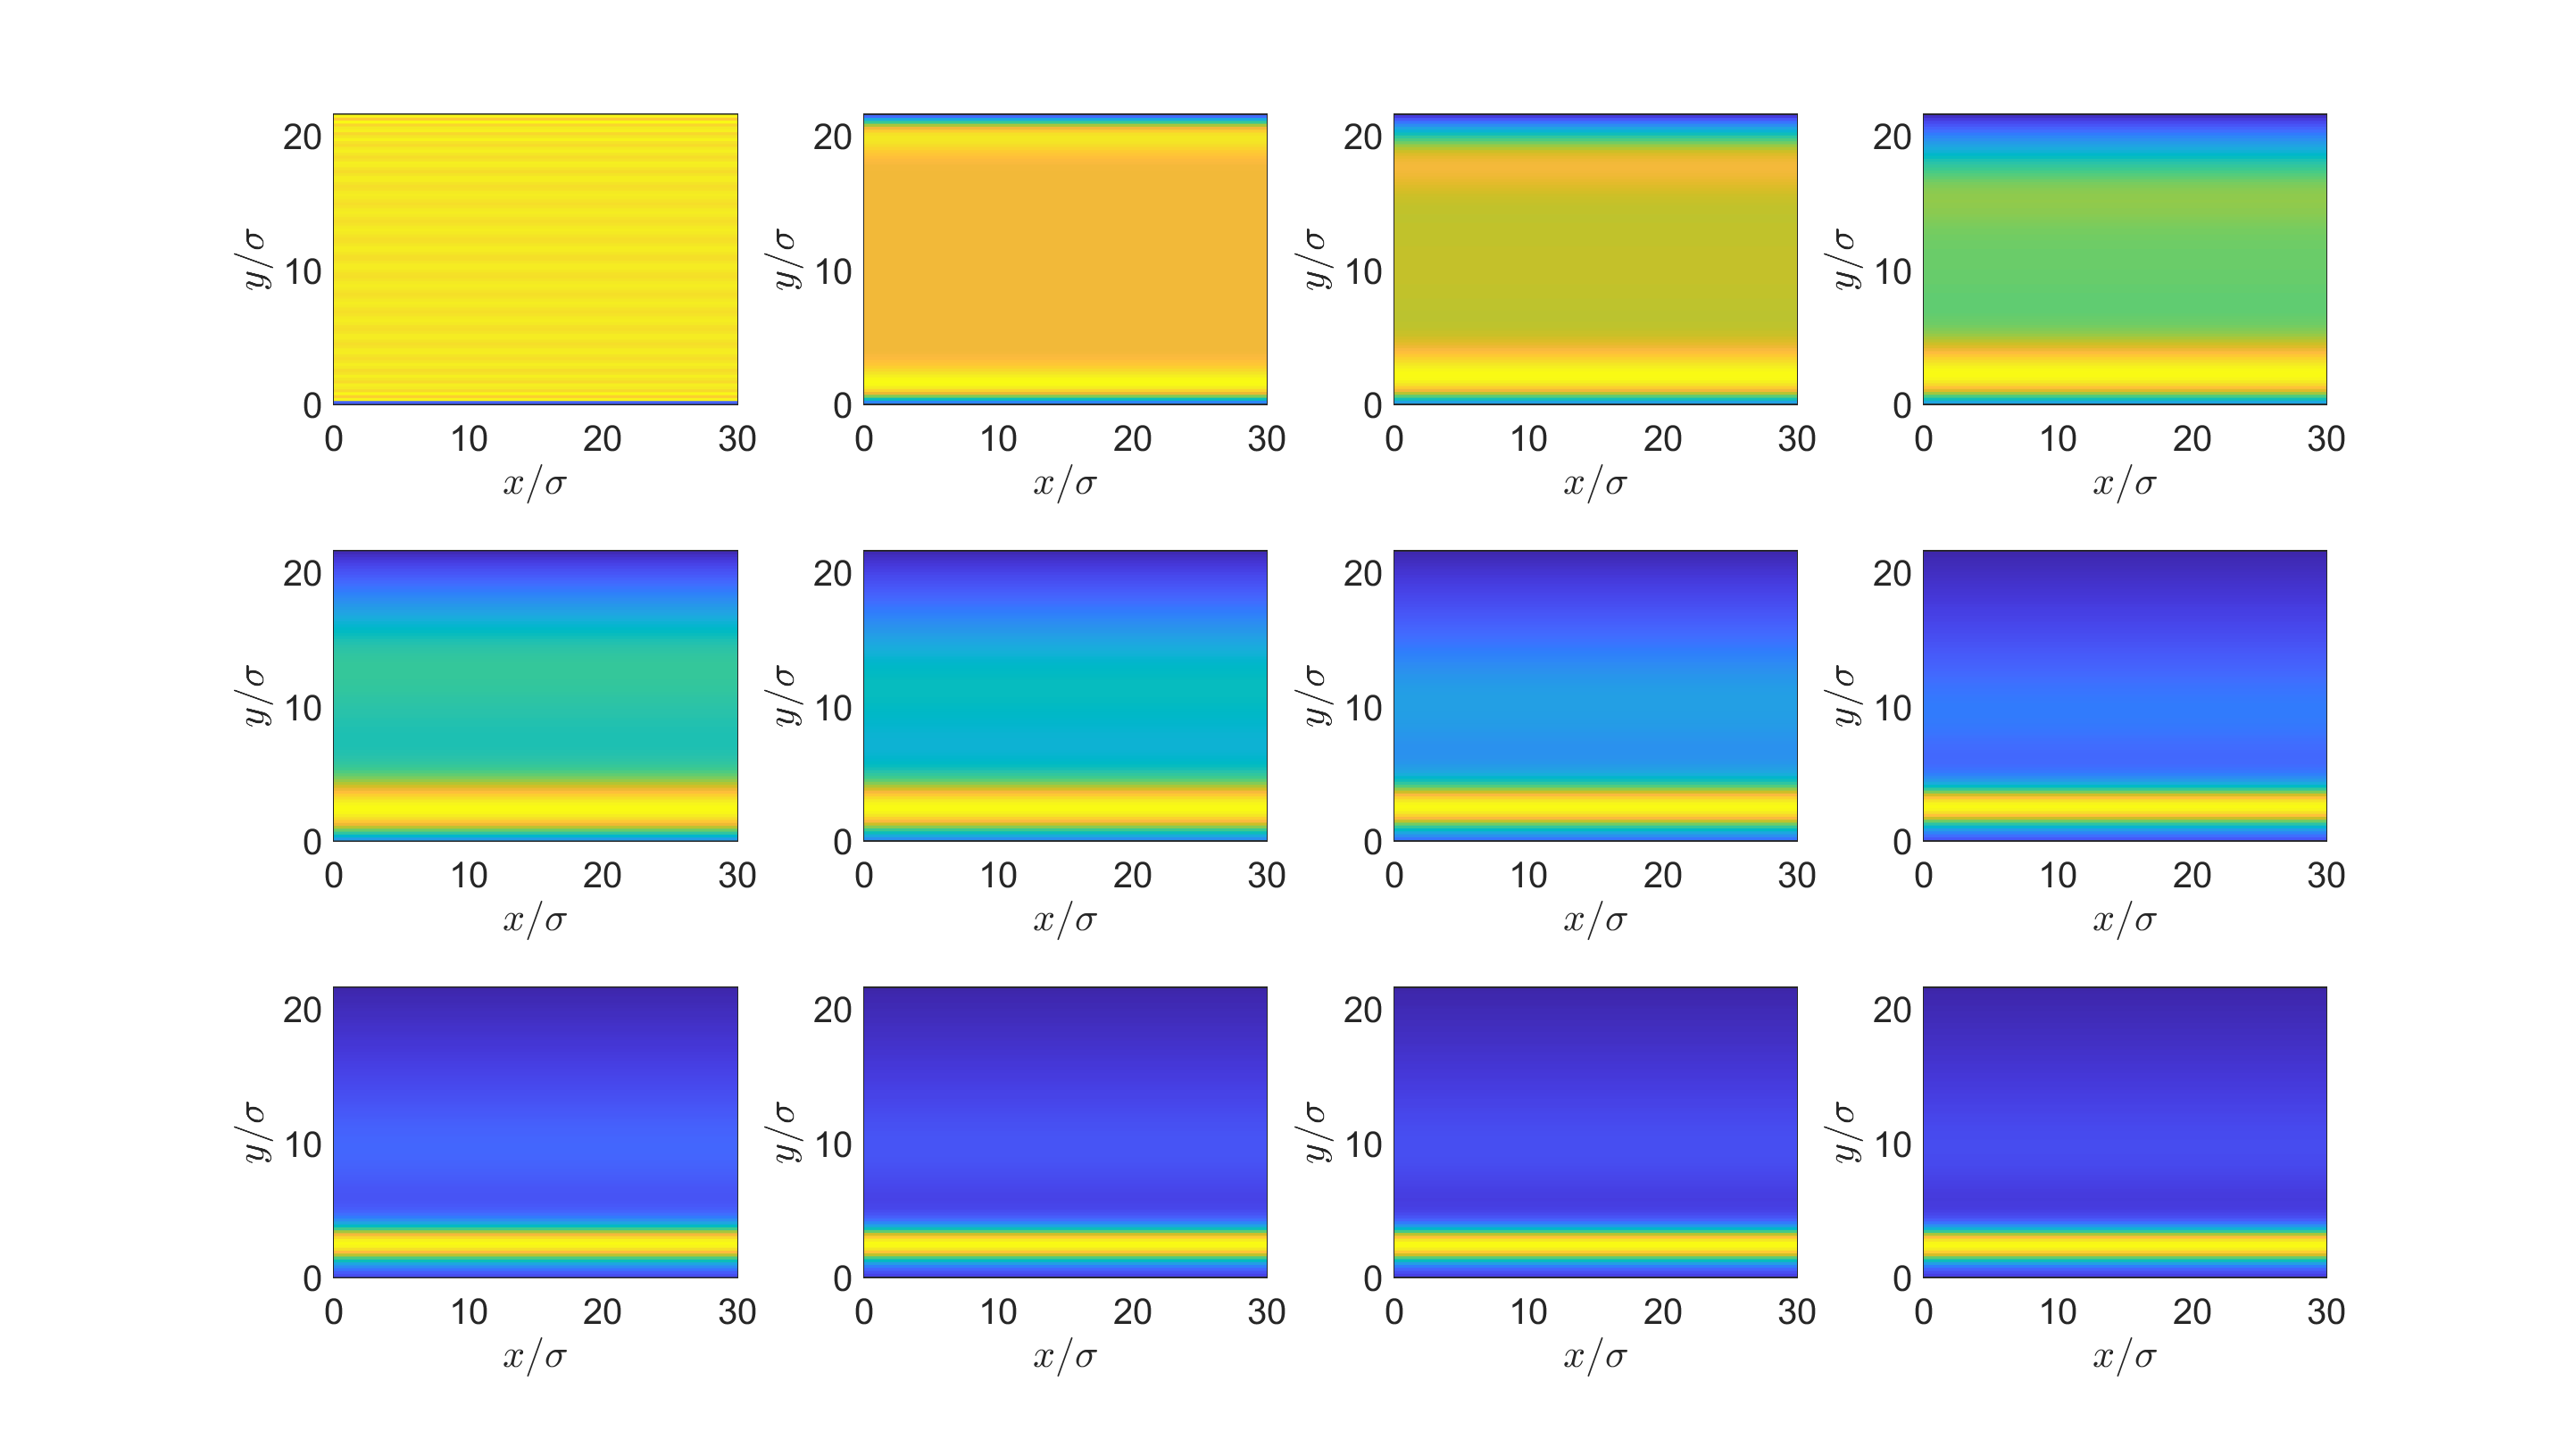
\includegraphics[scale=0.25]{Periodic2.png}
		\caption{$\sigma =0.5$, $\bar \rho =0.072$} 
		\label{F5}
	\end{figure}
	
	Then we consider $\sigma = 1$ and $\bar \rho = 0.2$, see Figure \ref{F6}.
	\begin{figure}[h]
		\centering
		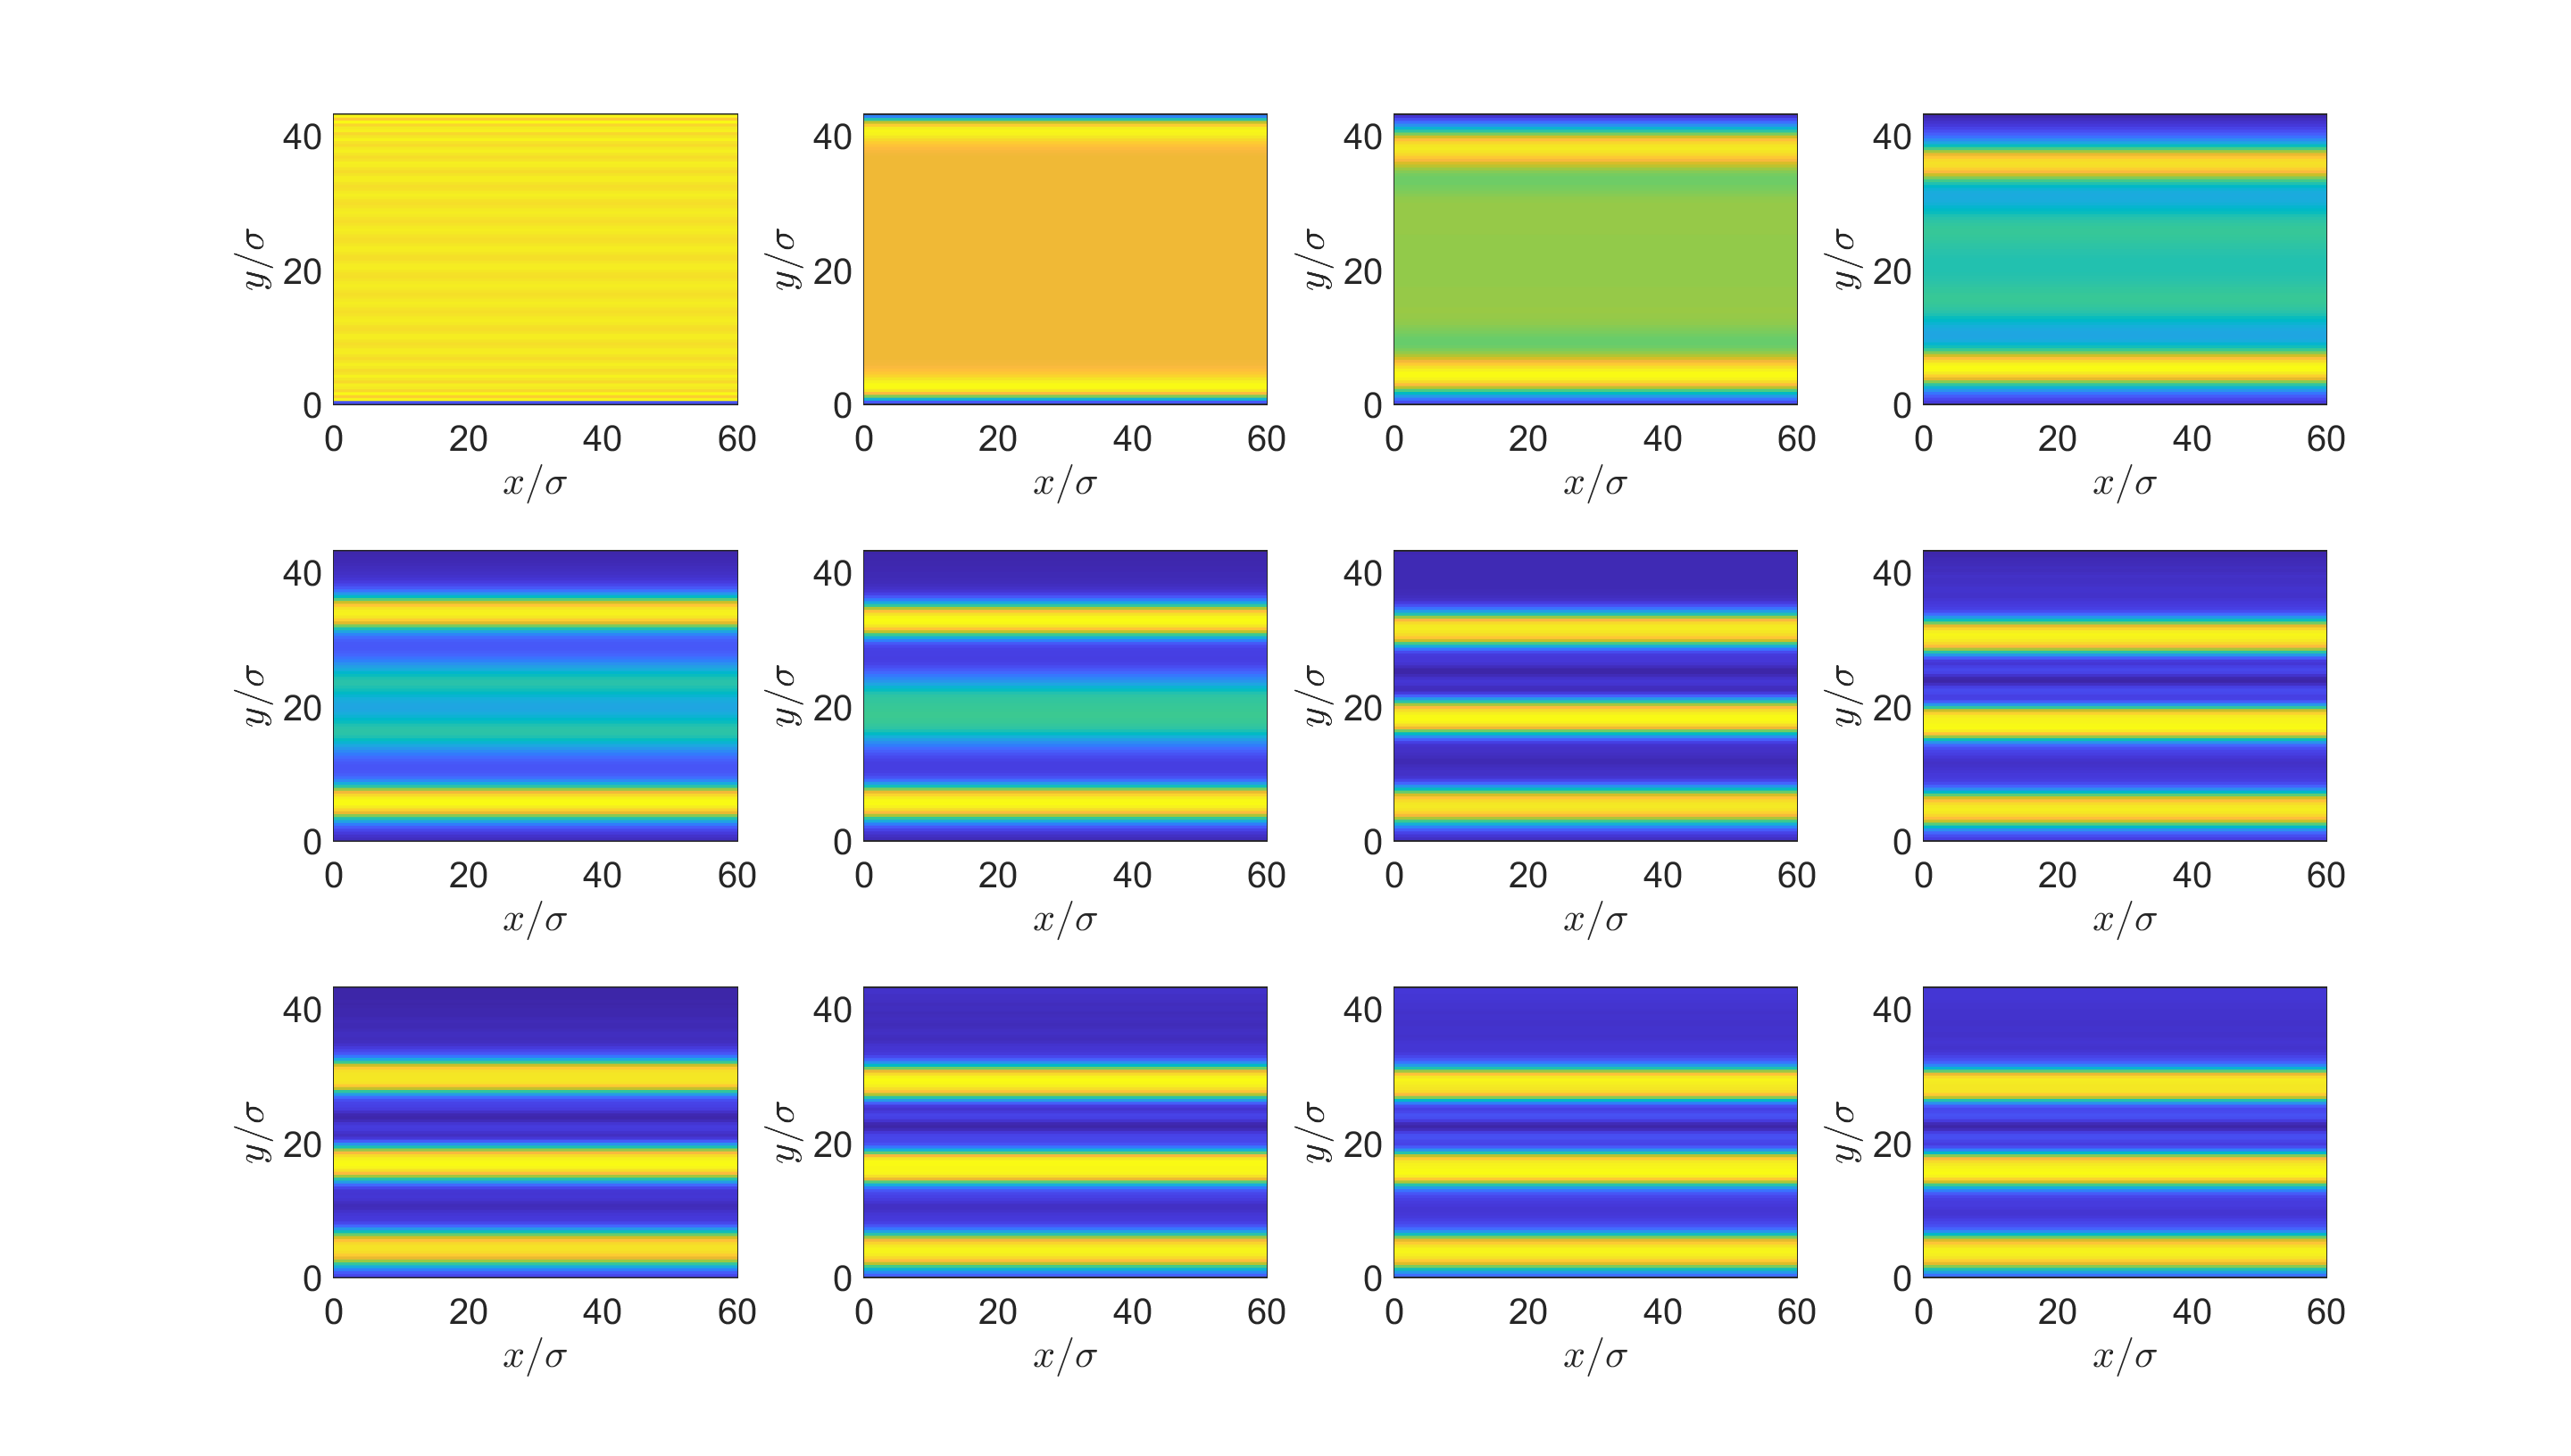
\includegraphics[scale=0.25]{Periodic3.png}
		\caption{$\sigma =1$, $\bar \rho =0.2$} 
		\label{F6}
	\end{figure}
	Then we consider $\sigma = 0.5$ and $\bar \rho = 0.2$, see Figure \ref{F7}.
	\begin{figure}[h]
		\centering
		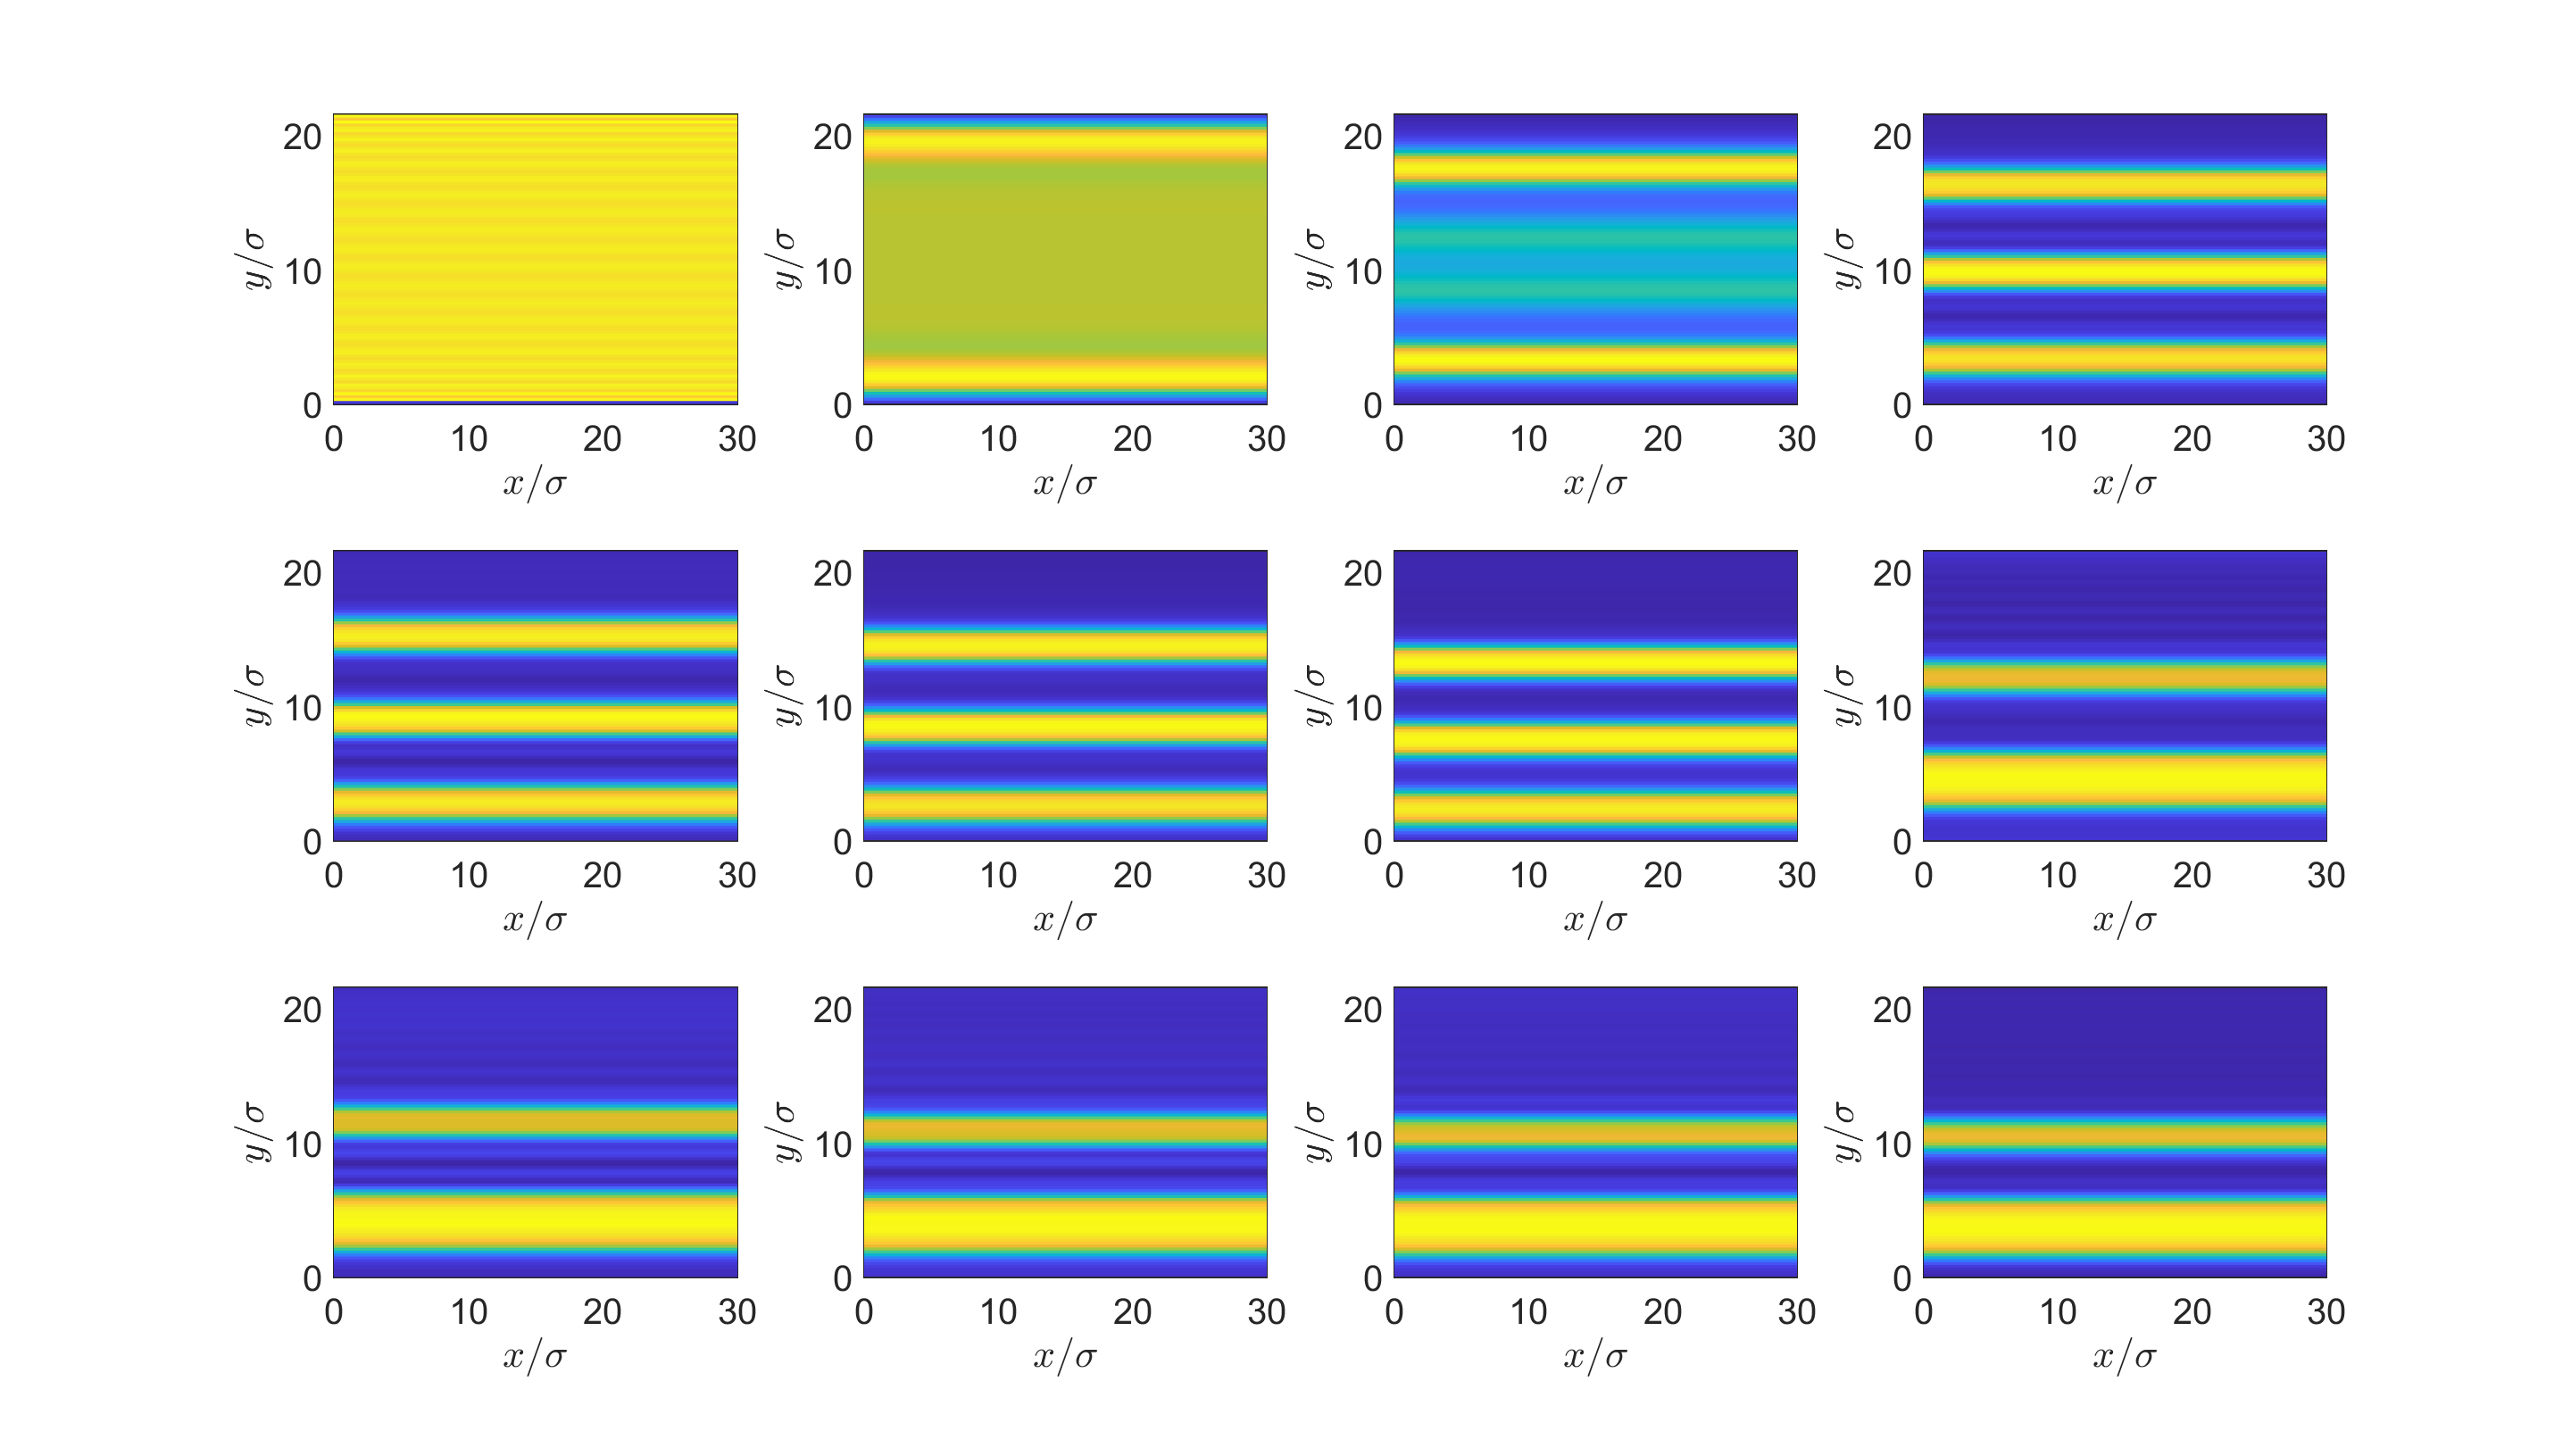
\includegraphics[scale=0.25]{Periodic4.png}
		\caption{$\sigma =0.5$, $\bar \rho =0.2$} 
		\label{F7}
	\end{figure}
	
	
\section{Sedimentation Multishape}
One odd thing here is that using Archer's interaction potential	two shapes are treated separately.This also happens when we use the Gaussian potential.
The two potentials are:
\begin{align*}
	V_A &= \exp(-y / \sigma)\\
	V_G &= \exp(-y^2).
\end{align*}
I am using two quadrilaterals and the external potential is acting downward as before, $n = 20$ and for each shape $N = 30$. 
Using $V_A$ is displayed in Figure \ref{F8} and using $V_9$ is displayed in Figure \ref{F9}. But looks like my problem is solved now... see Figure \ref{F9b}.
\begin{figure}[h]
	\centering
	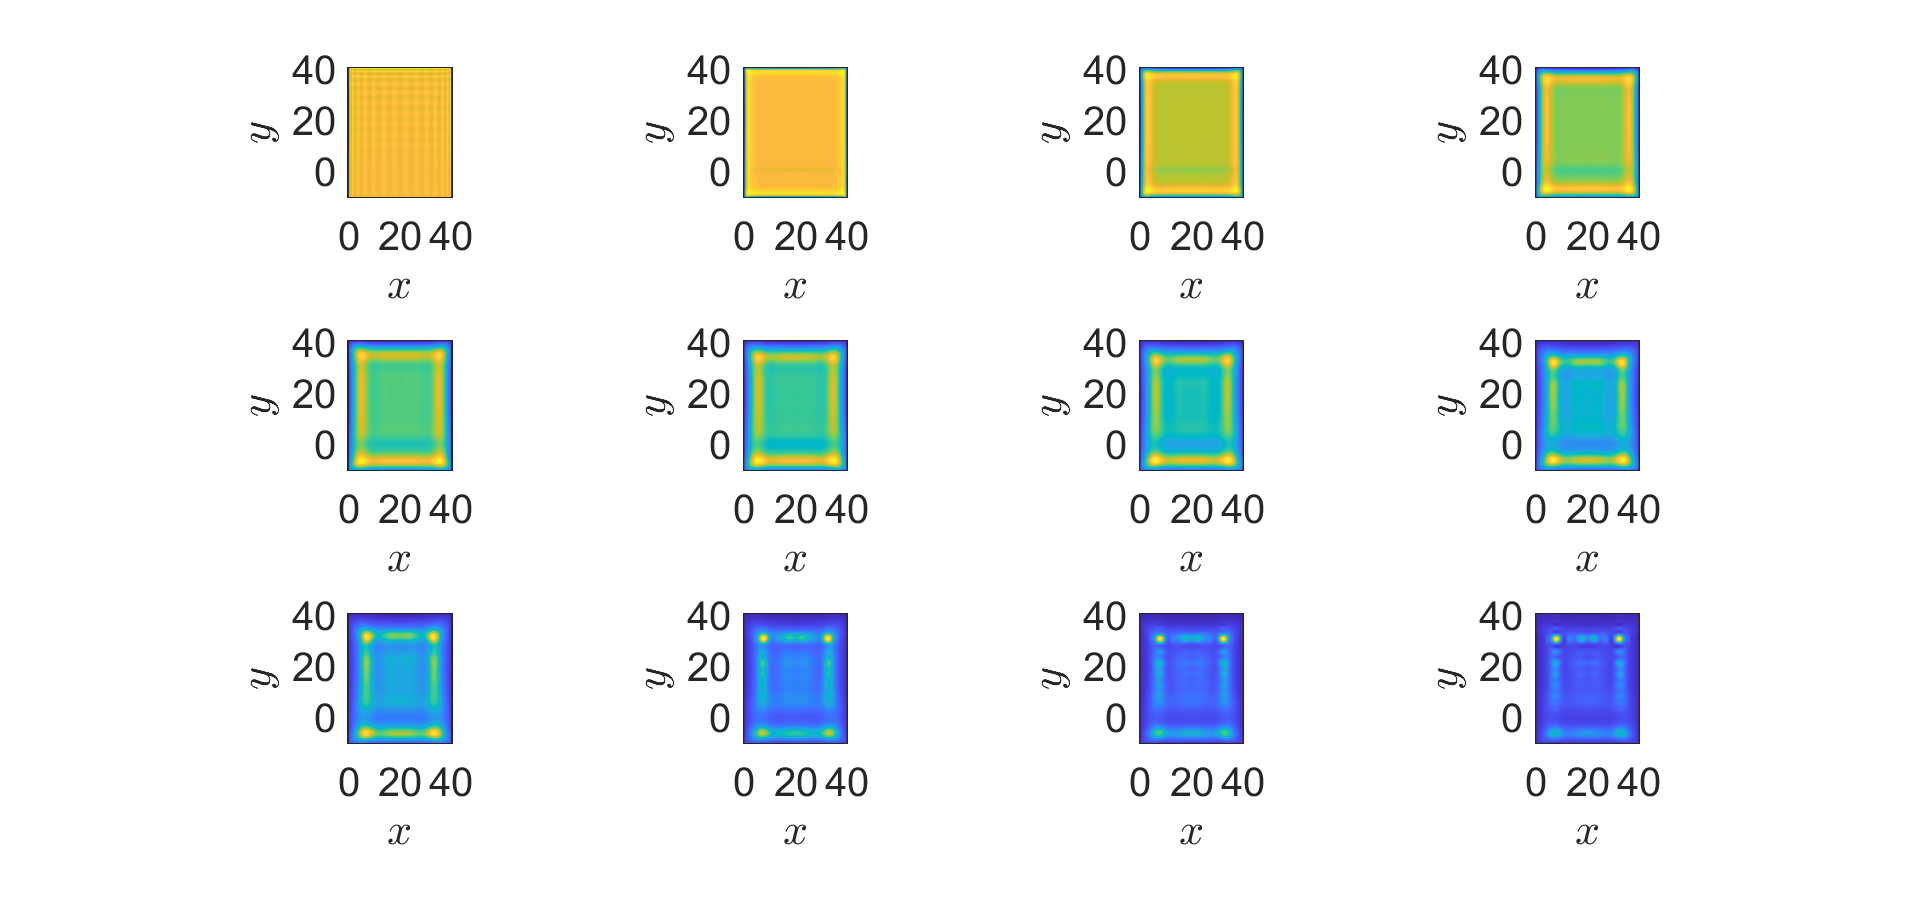
\includegraphics[scale=0.4]{Multi1.png}
	\caption{$\sigma =1$, $\bar \rho =0.072$, $TMax = 20$, $V_A$} 
	\label{F8}
\end{figure}

\begin{figure}[h]
	\centering
	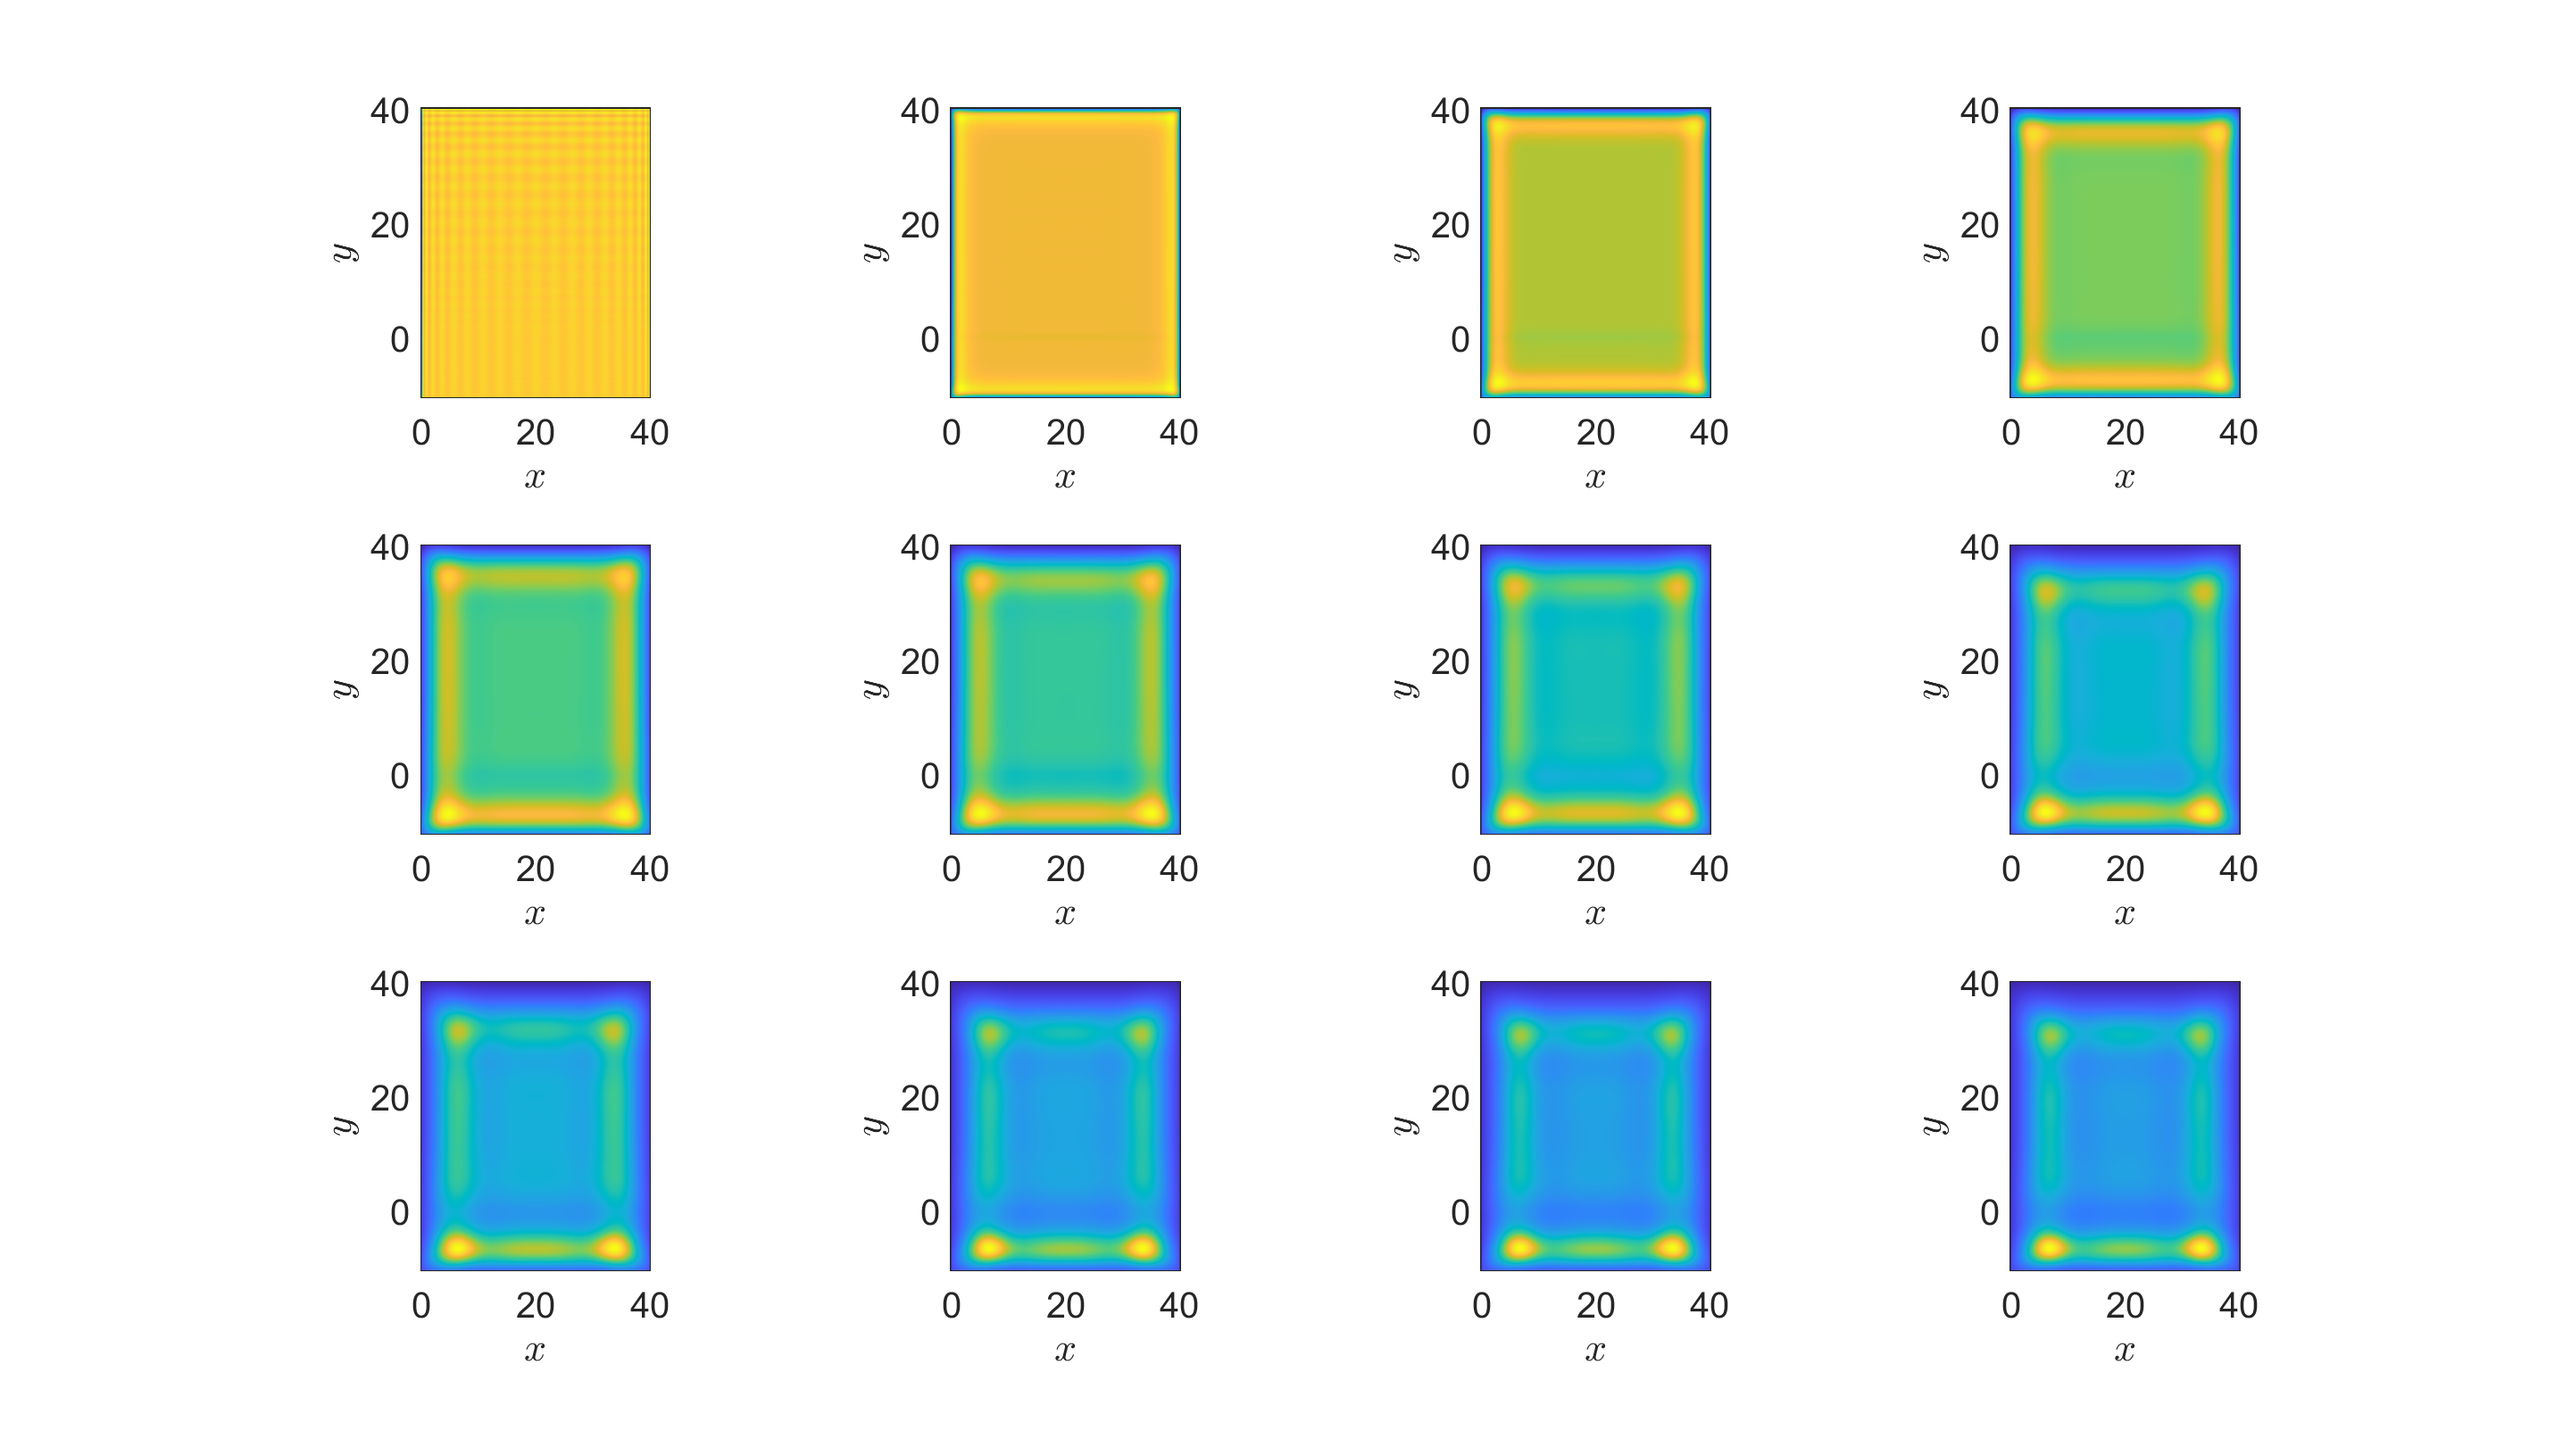
\includegraphics[scale=0.25]{MultiSolve1.png}
	\caption{$\sigma =1$, $\bar \rho =0.072$, $TMax = 20$, $V_A$ more points} 
	\label{F9b}
\end{figure}
\begin{figure}[h]
	\centering
	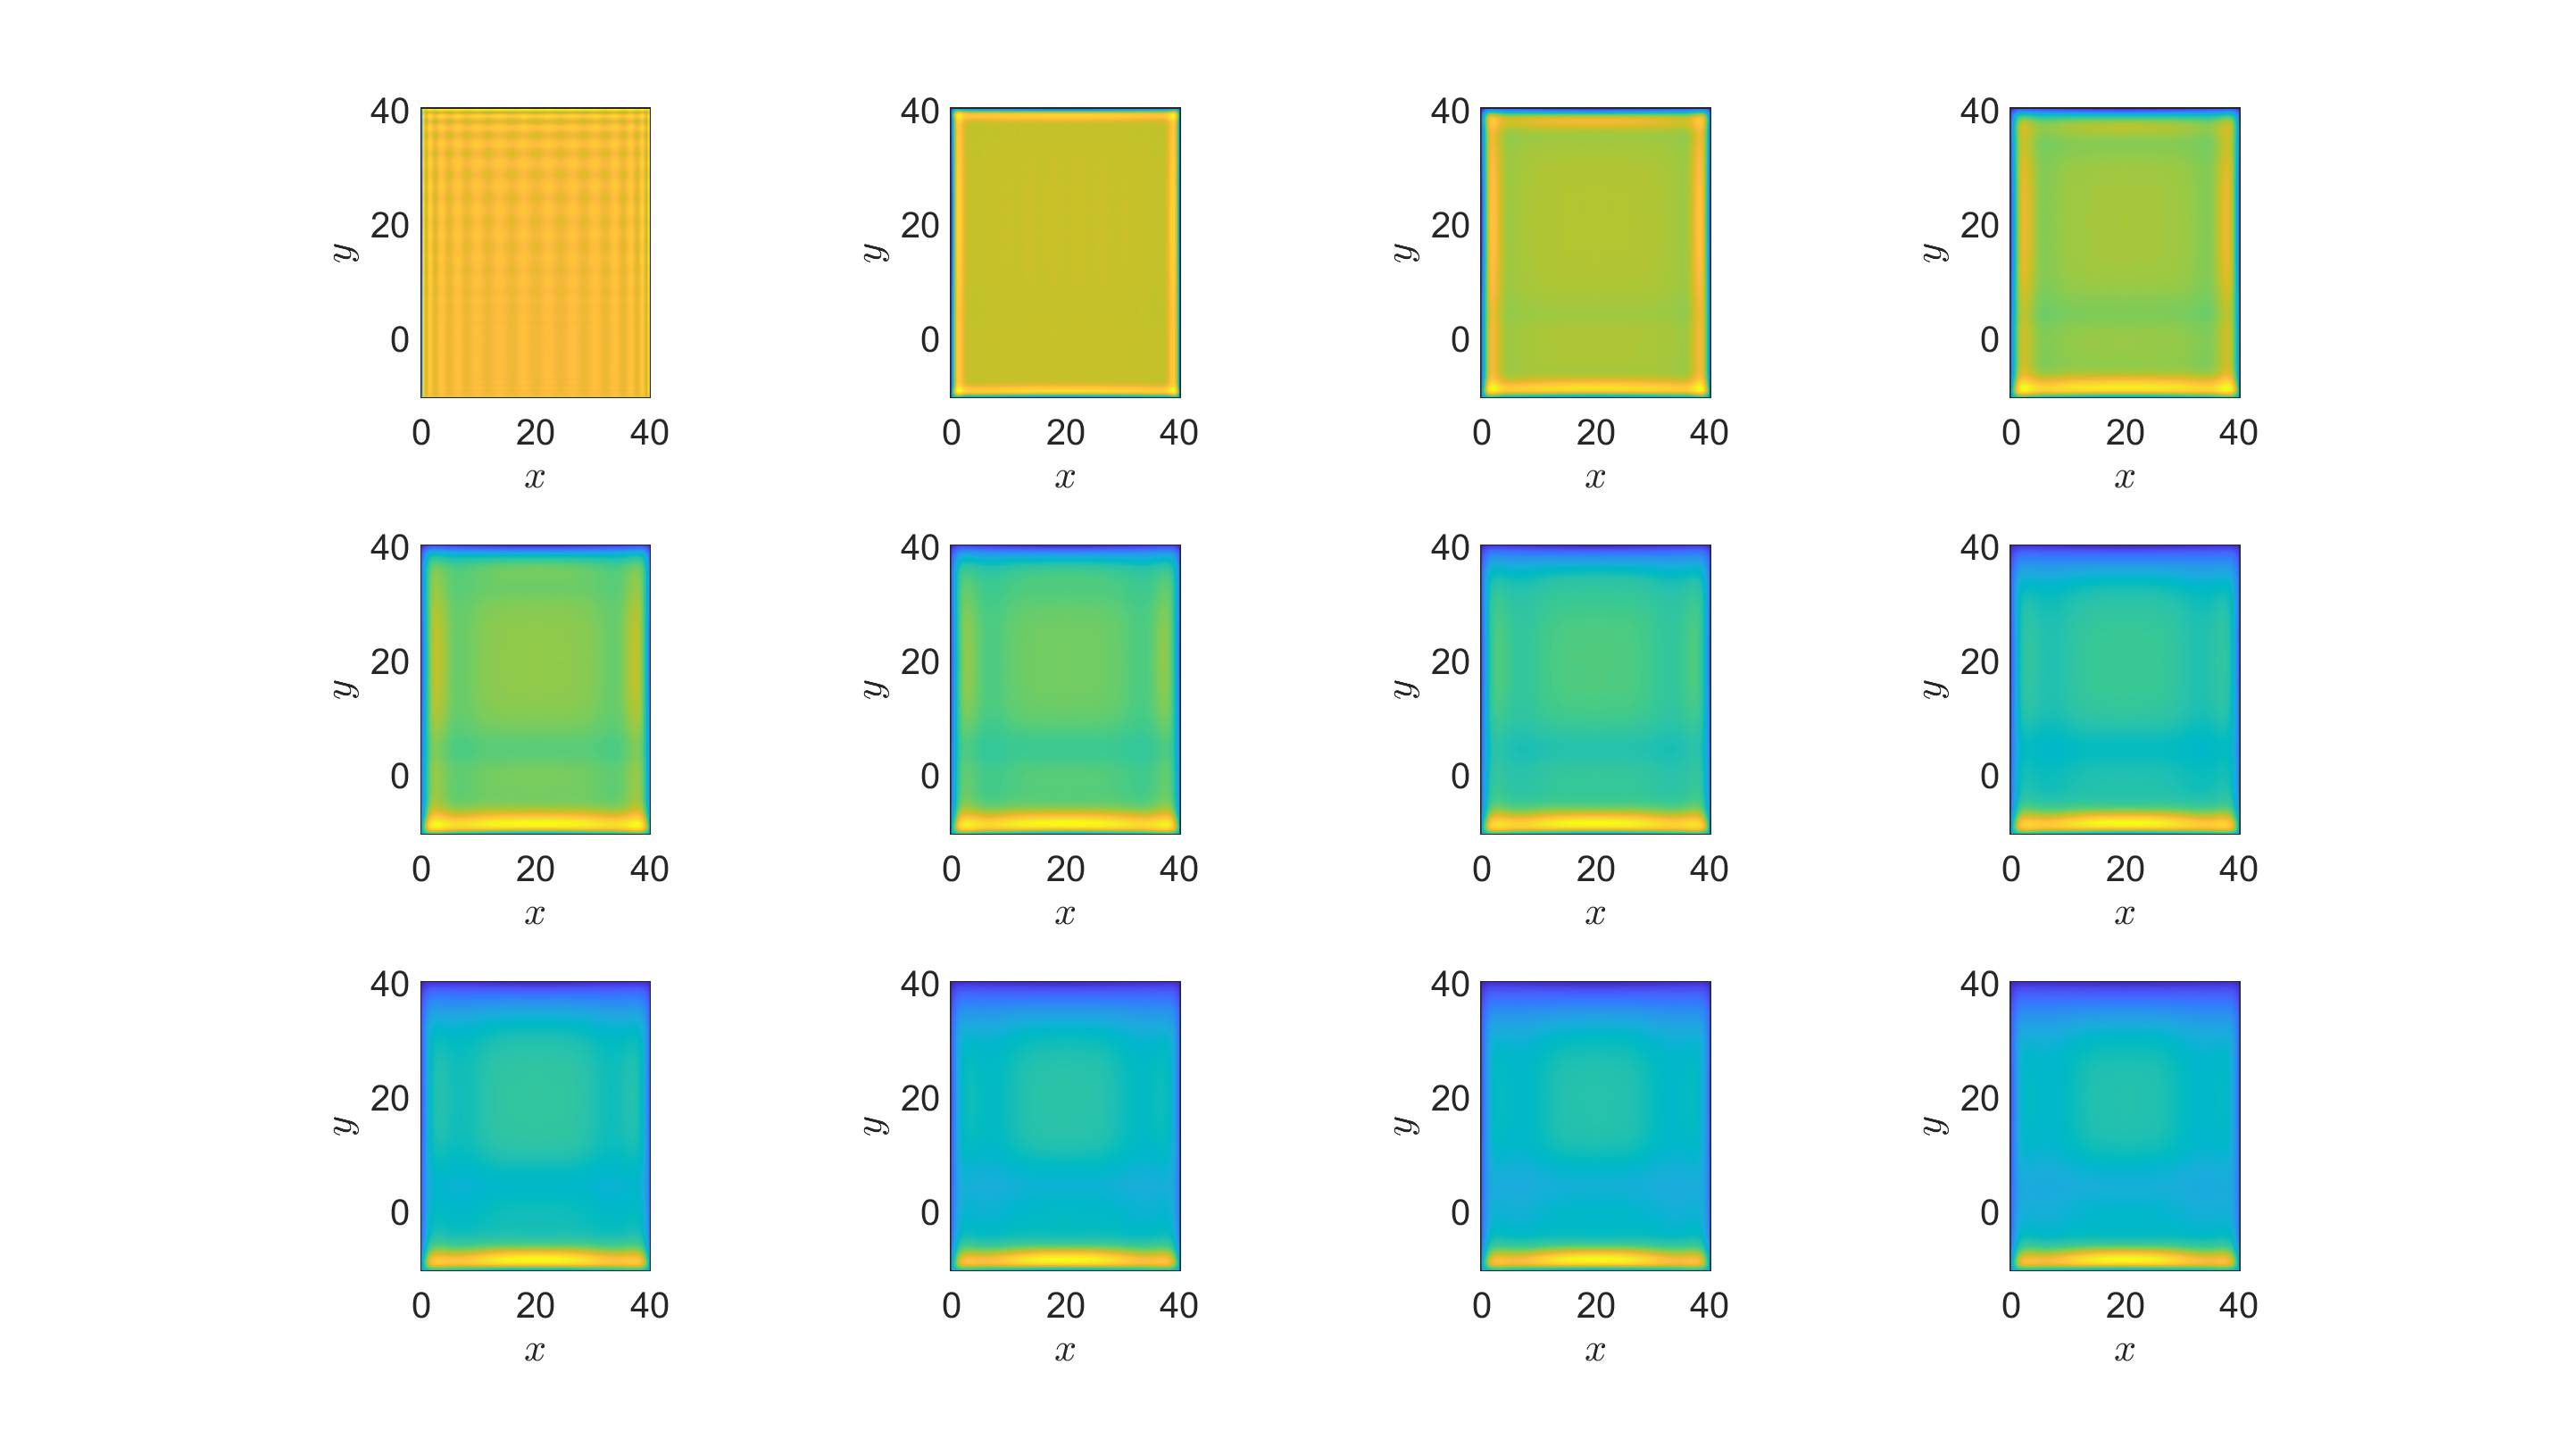
\includegraphics[scale=0.25]{Multi2.png}
	\caption{$\sigma =1$, $\bar \rho =0.072$, $TMax = 20$, $V_G$} 
	\label{F9}
\end{figure}
When using $\bar \rho = 0.2$, the code breaks due to lack of points I think. 
When $\bar \rho = 0.0001$, we get smooth behaviour in both.
So if that is the only problem then we can make some pretty plots for the sake of it, see Figure \ref{Fpp}.
\begin{figure}[h]
	\centering
	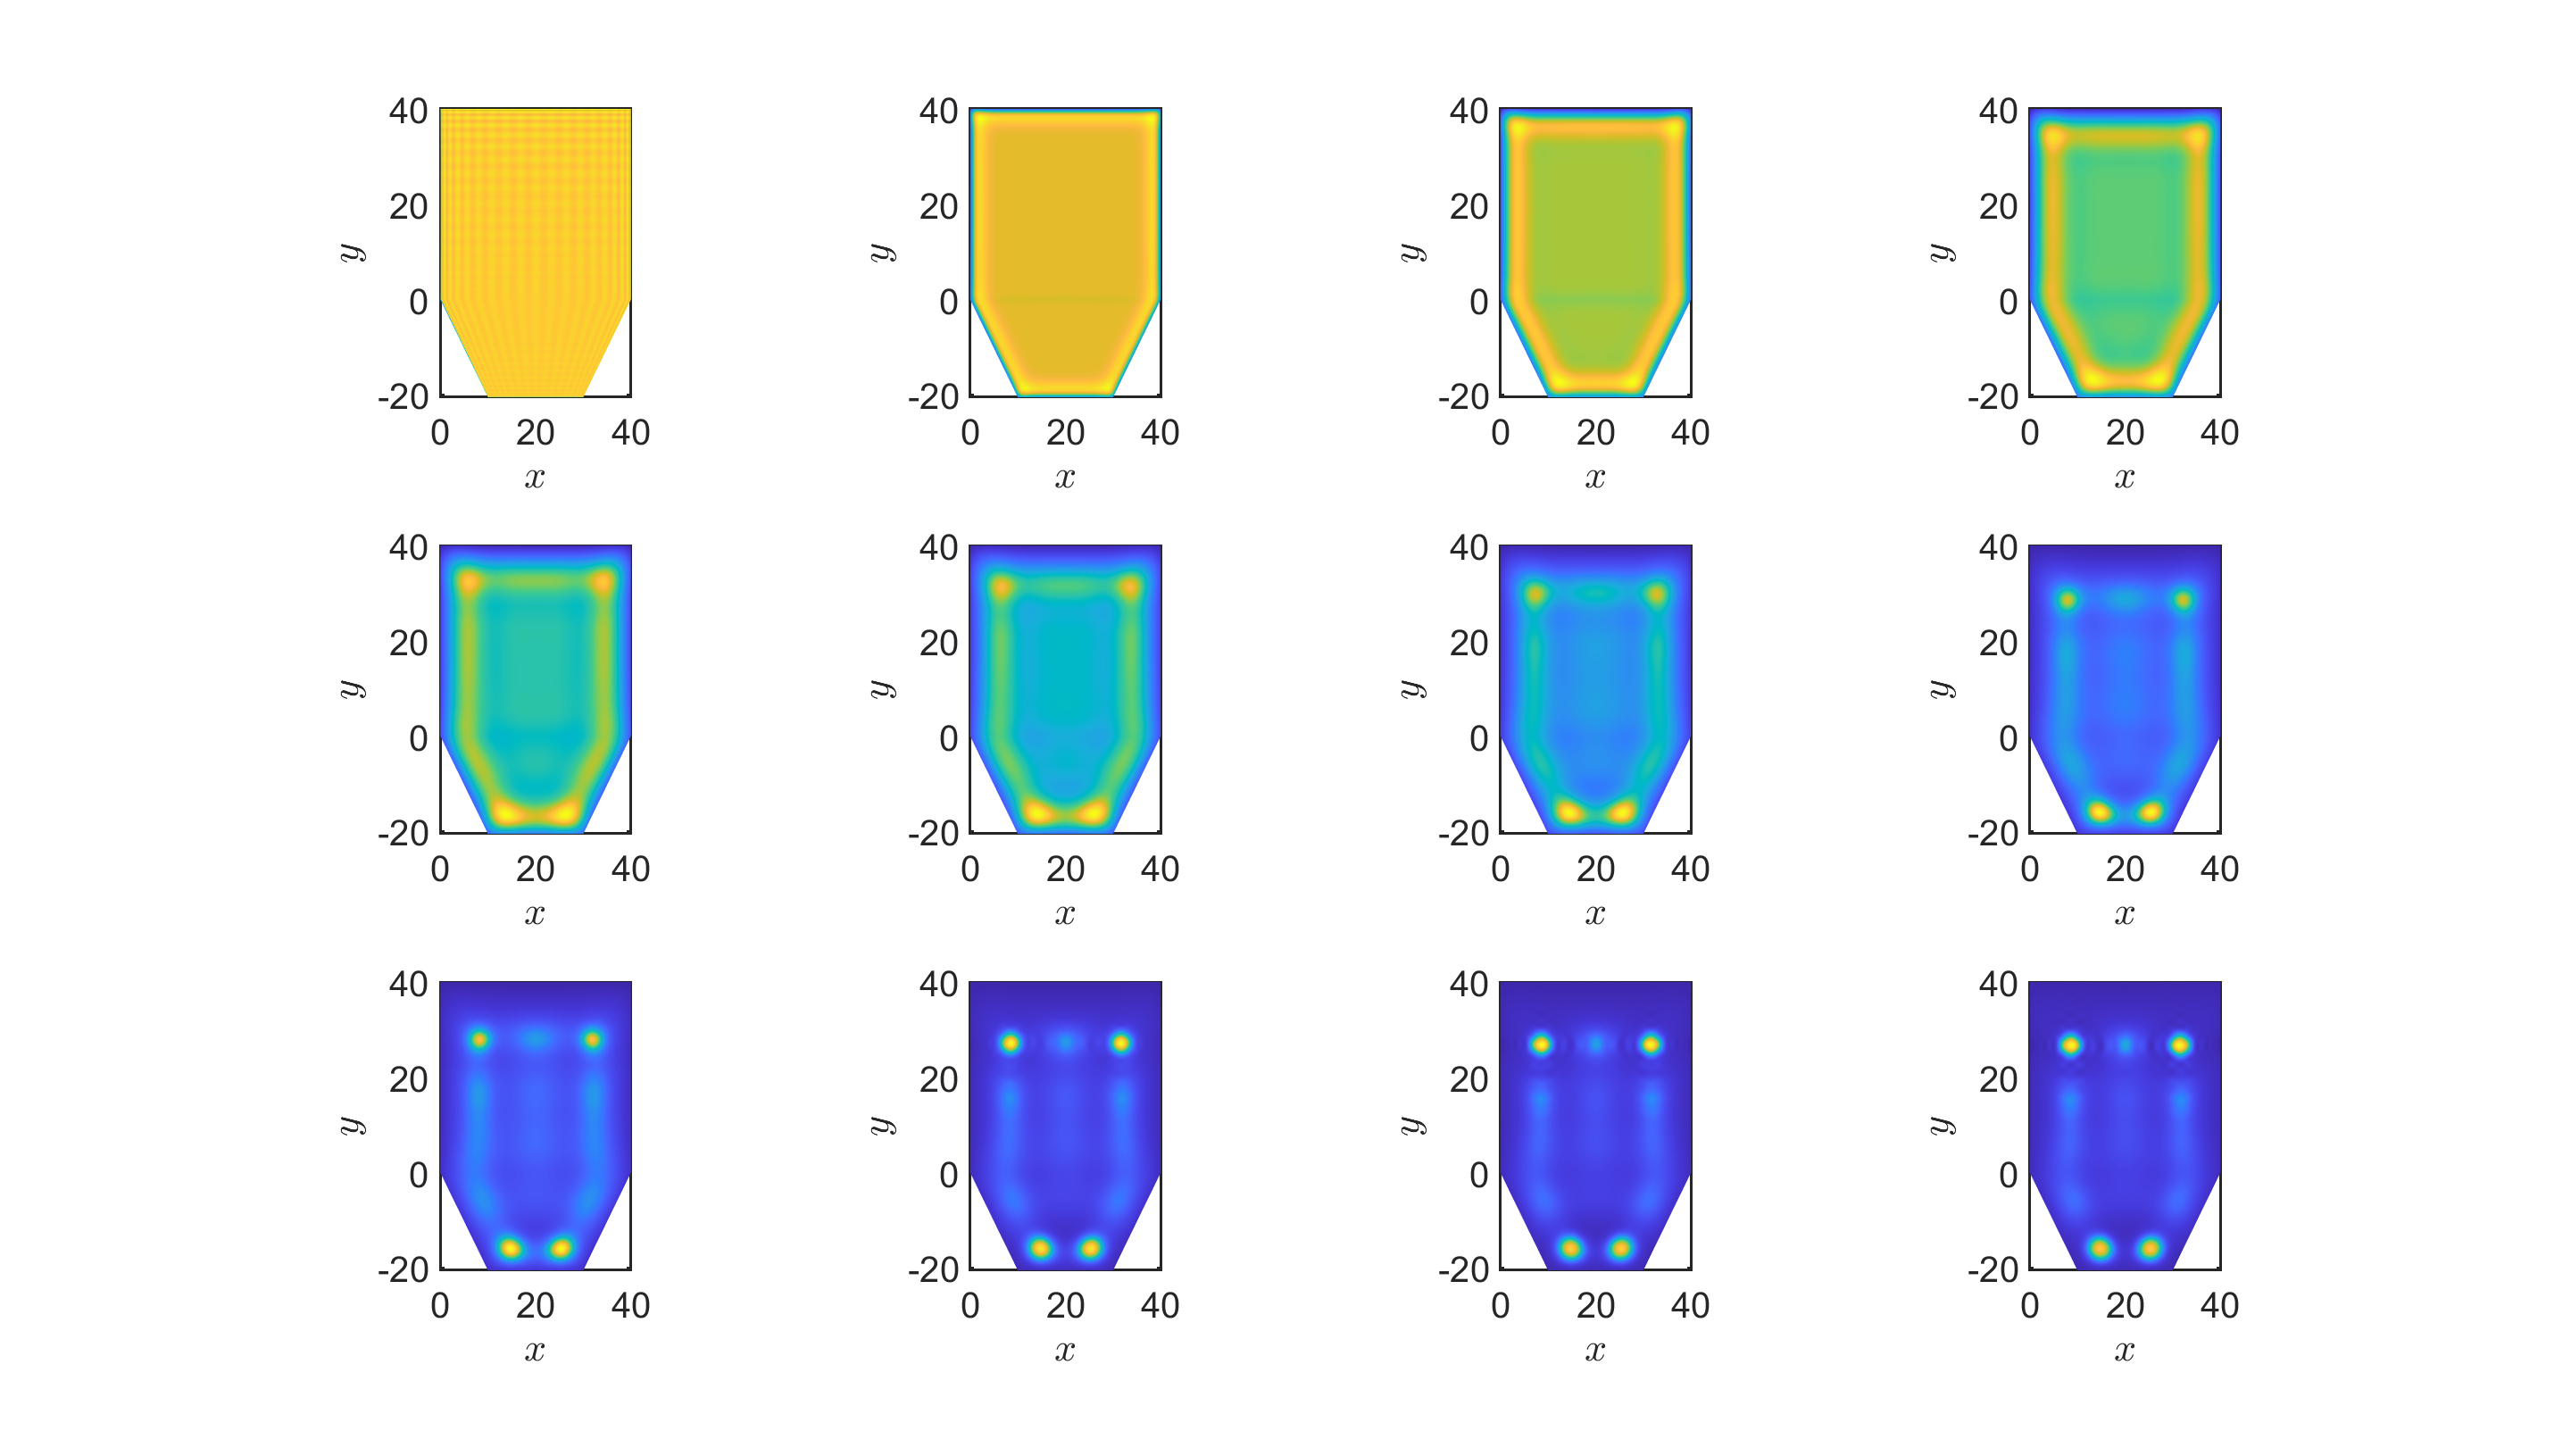
\includegraphics[scale=0.25]{PrettyPicture.png}
	\caption{$\sigma =1$, $\bar \rho =0.072$, $TMax = 40$, $V_A$} 
	\label{Fpp}
\end{figure}
\begin{figure}[h]
	\centering
	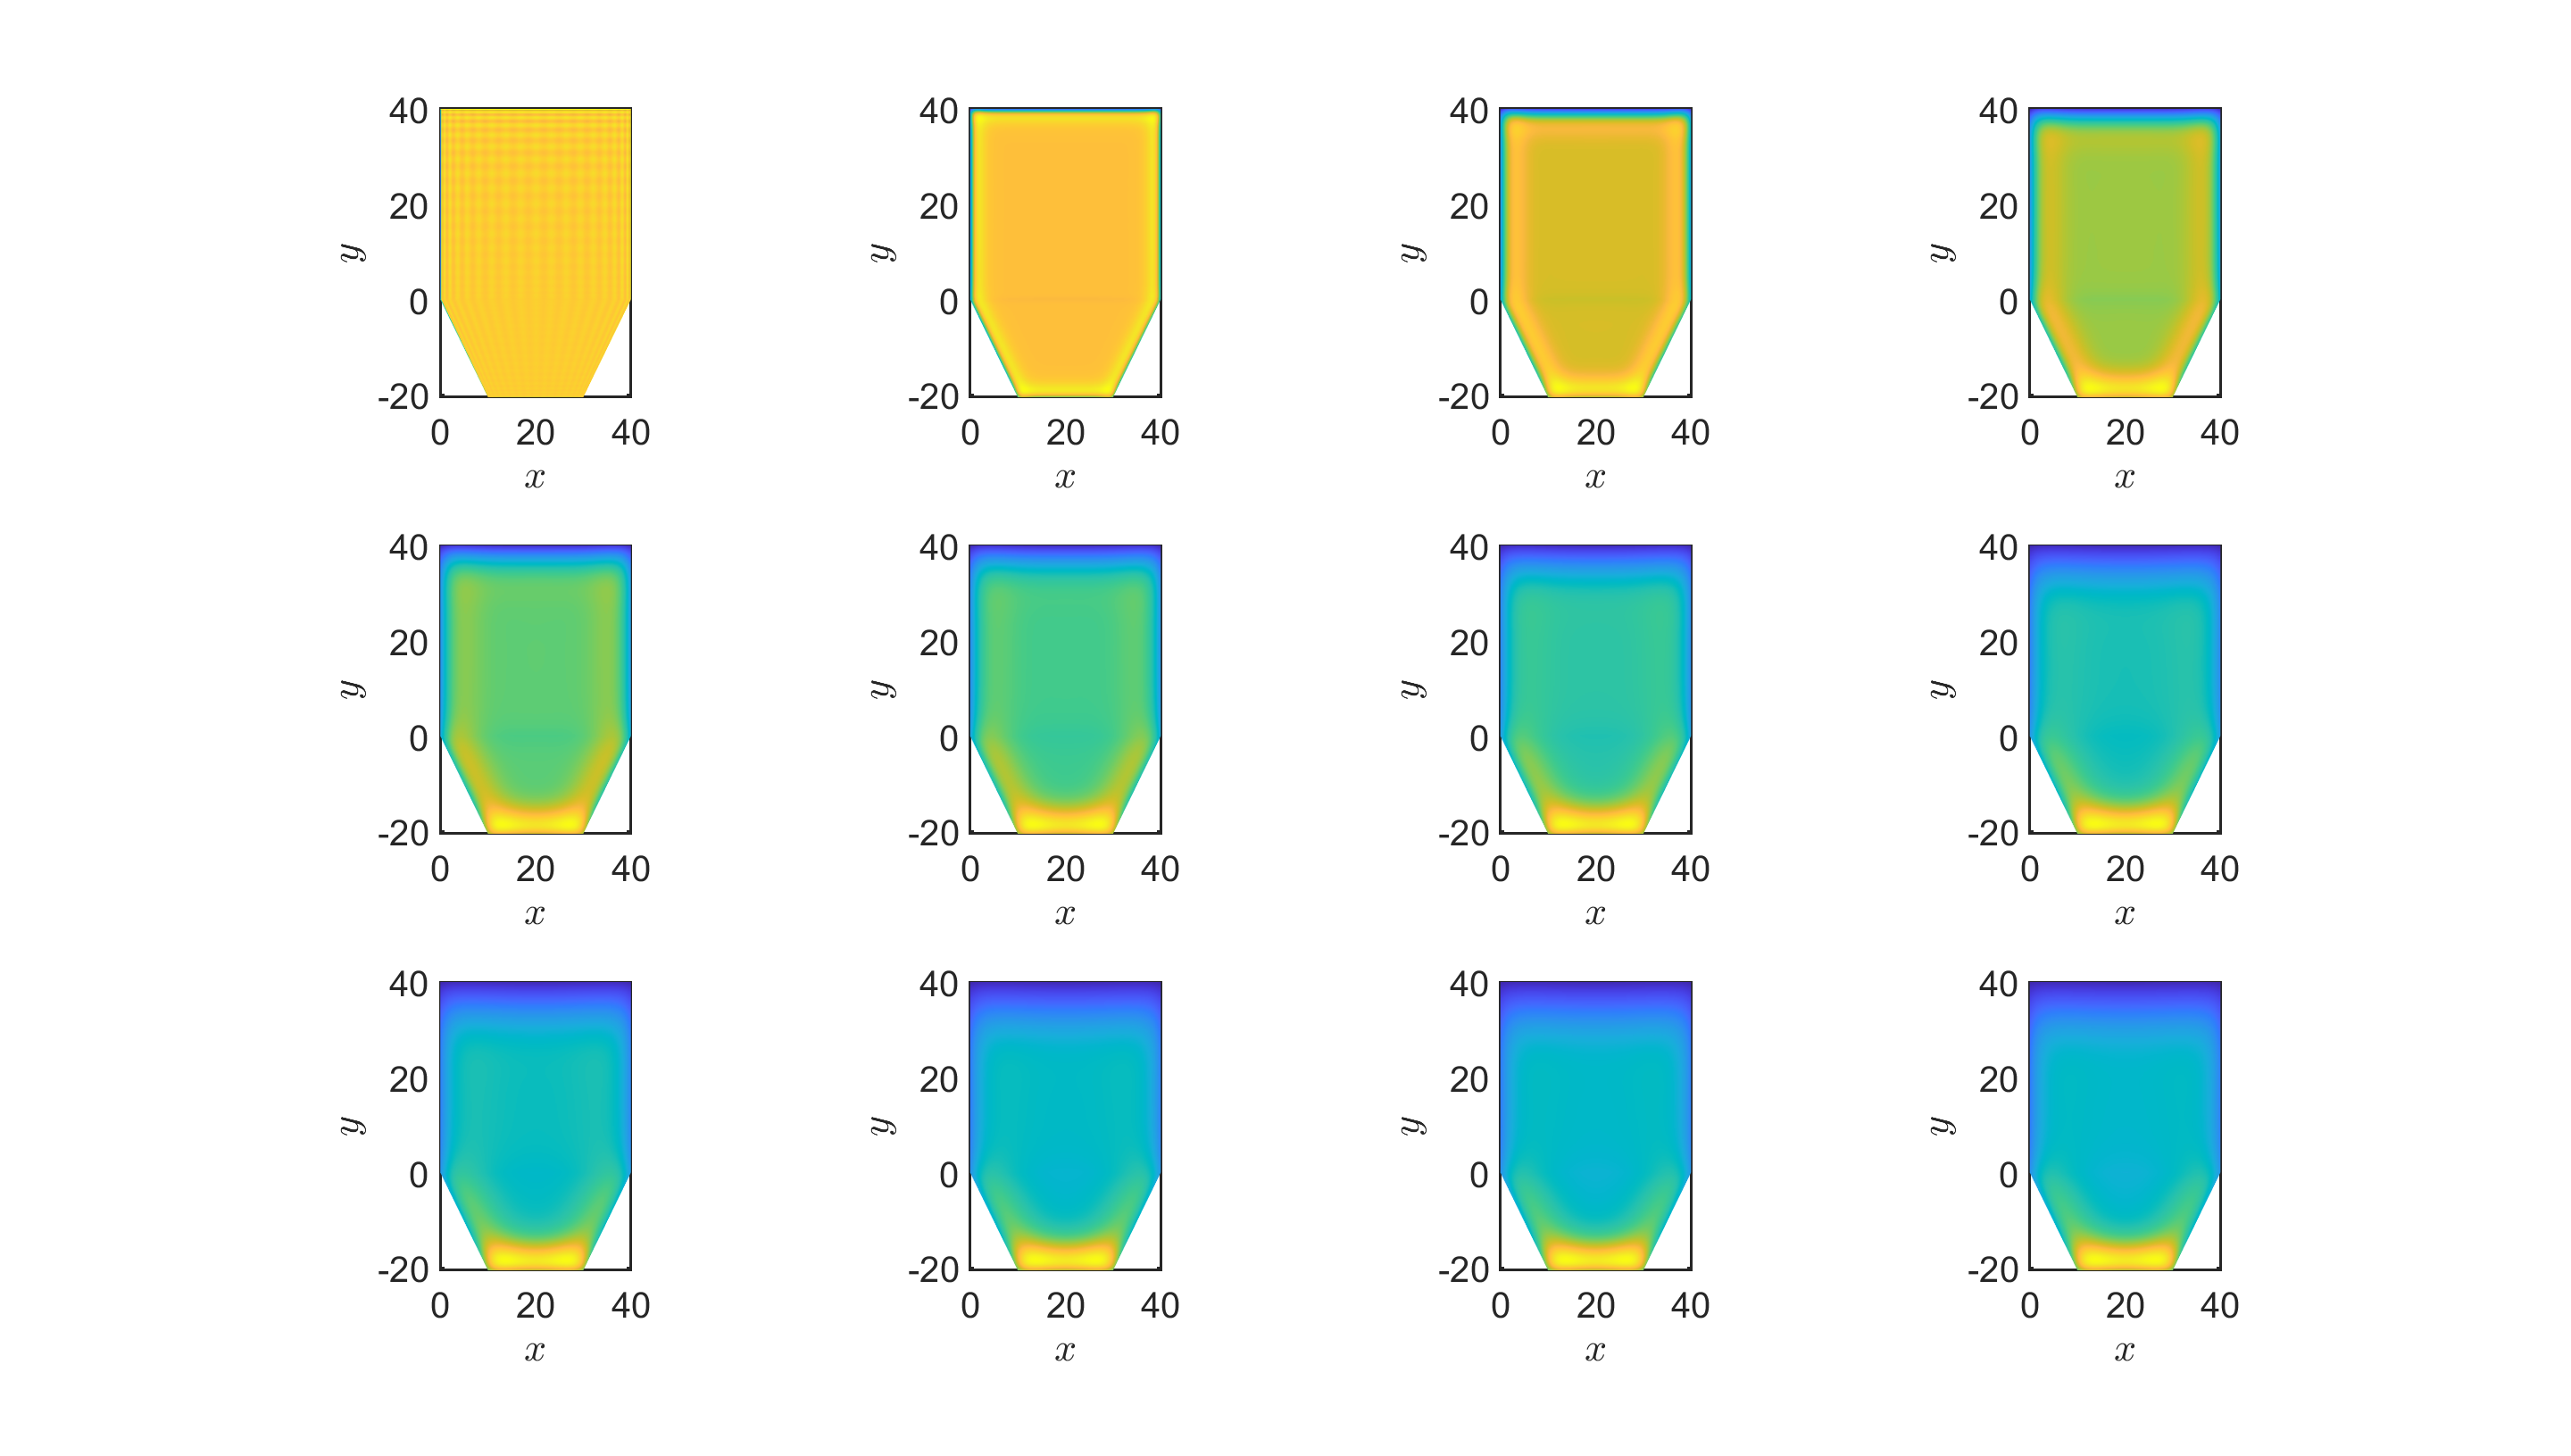
\includegraphics[scale=0.25]{PrettyPicture2.png}
	\caption{$\sigma =1$, $\bar \rho =0.05$, $TMax = 40$, $V_A$, less attraction ($\kappa = -2$)} 
	\label{Fpp2}
\end{figure}
\\
\\
Another weird thing, which doesn't have to do with the multishape is the inital condition for $\rho$. When plotting the solution for $\rho$ at time $0$, this is not uniform but influenced by $V_{ext}$ and $V_2$. We assumed that was due to the perturbation in $\rho_0$ but this is with uniform $\rho_0$. The different influences are displayed in Figure \ref{F10}. I guess these effects are normal though? 
\begin{figure}[h]
	\centering
	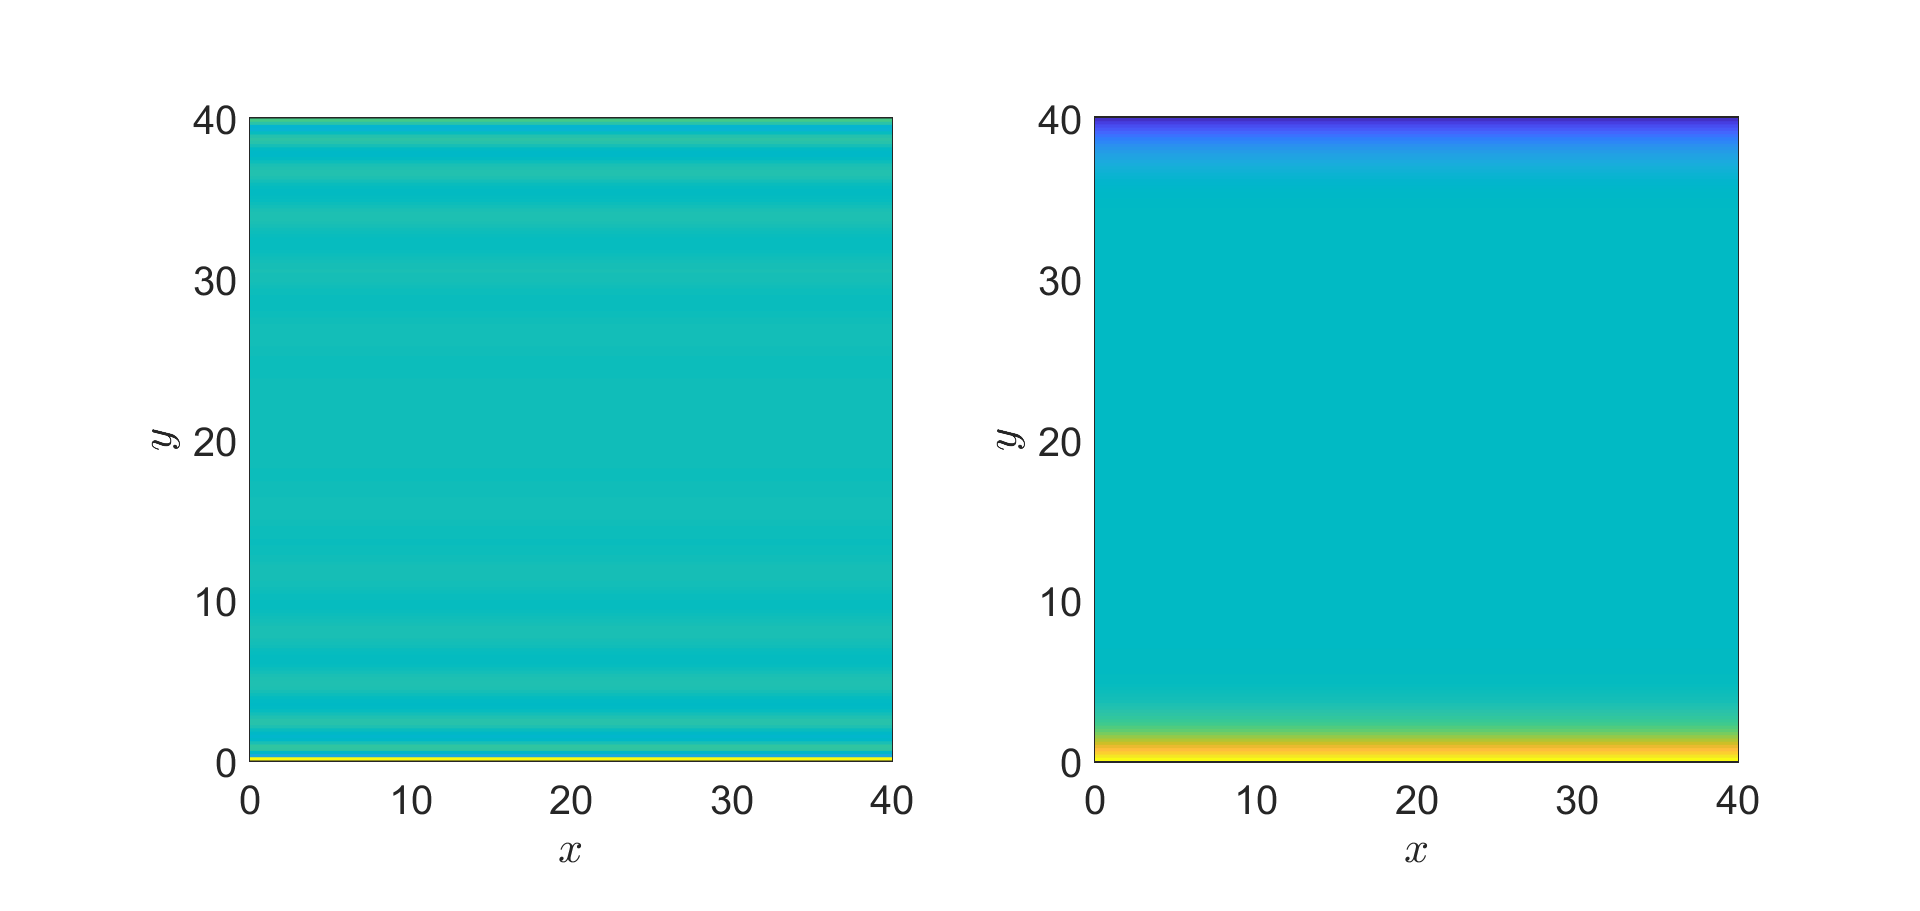
\includegraphics[scale=0.25]{OneShape1.png}
	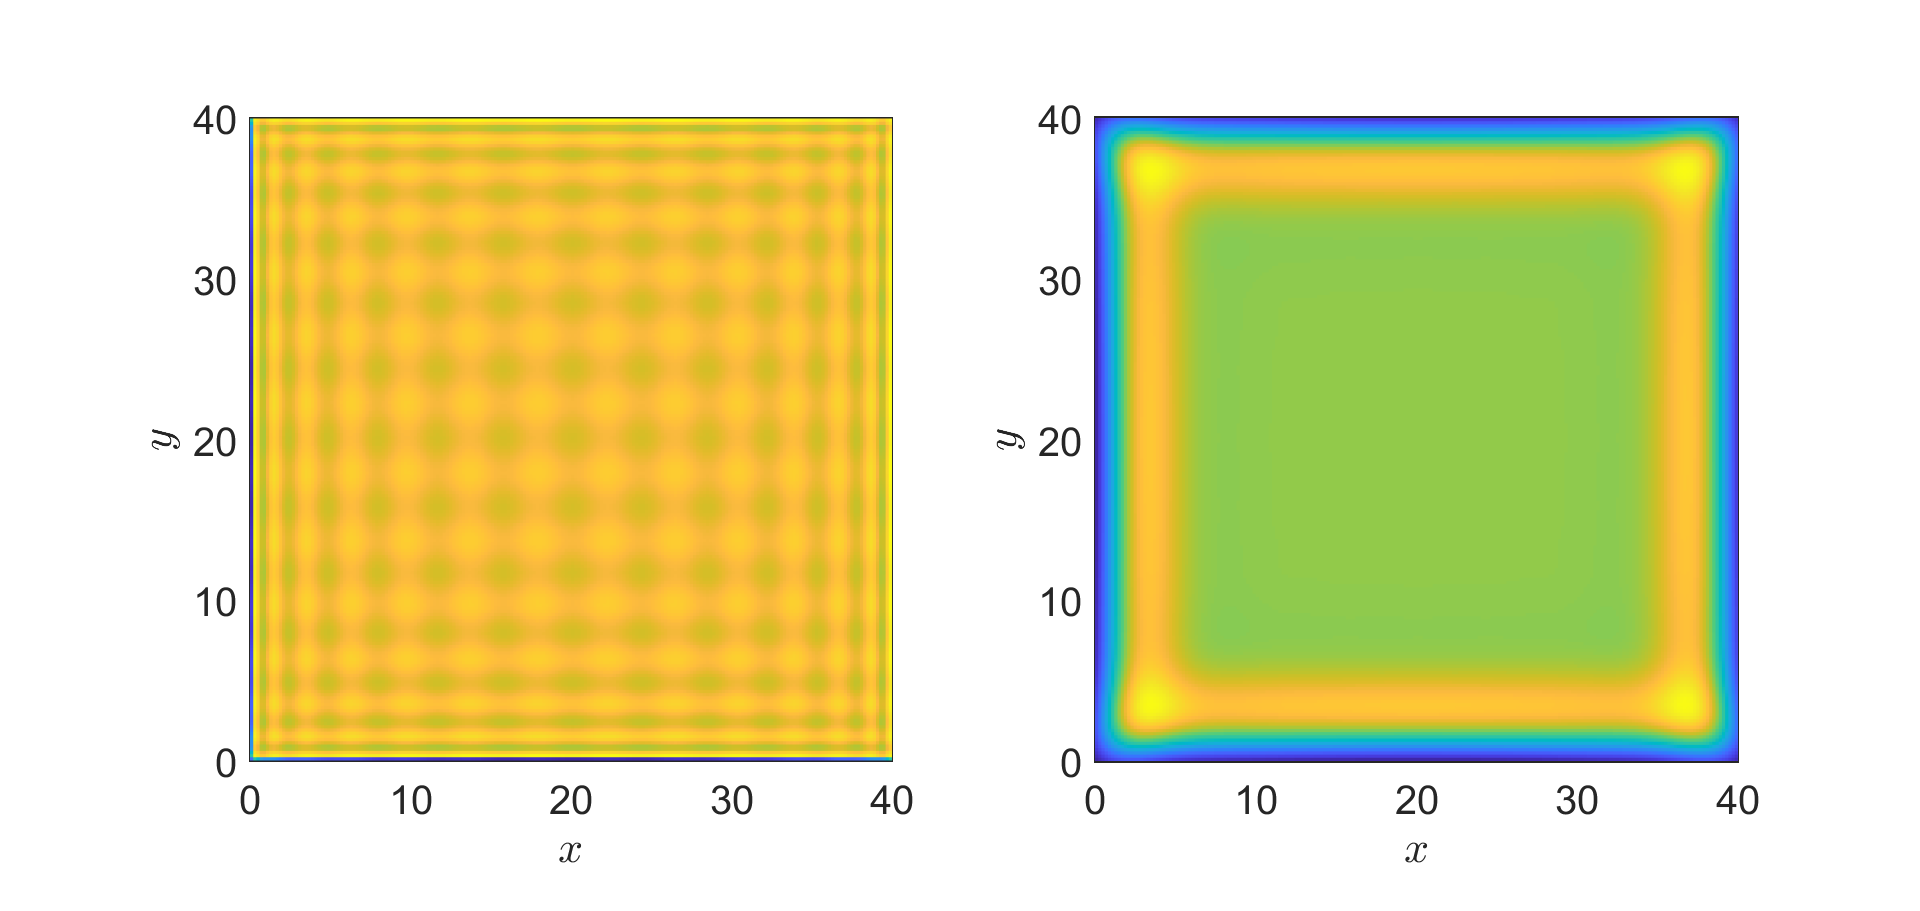
\includegraphics[scale=0.25]{OneShape2.png}
	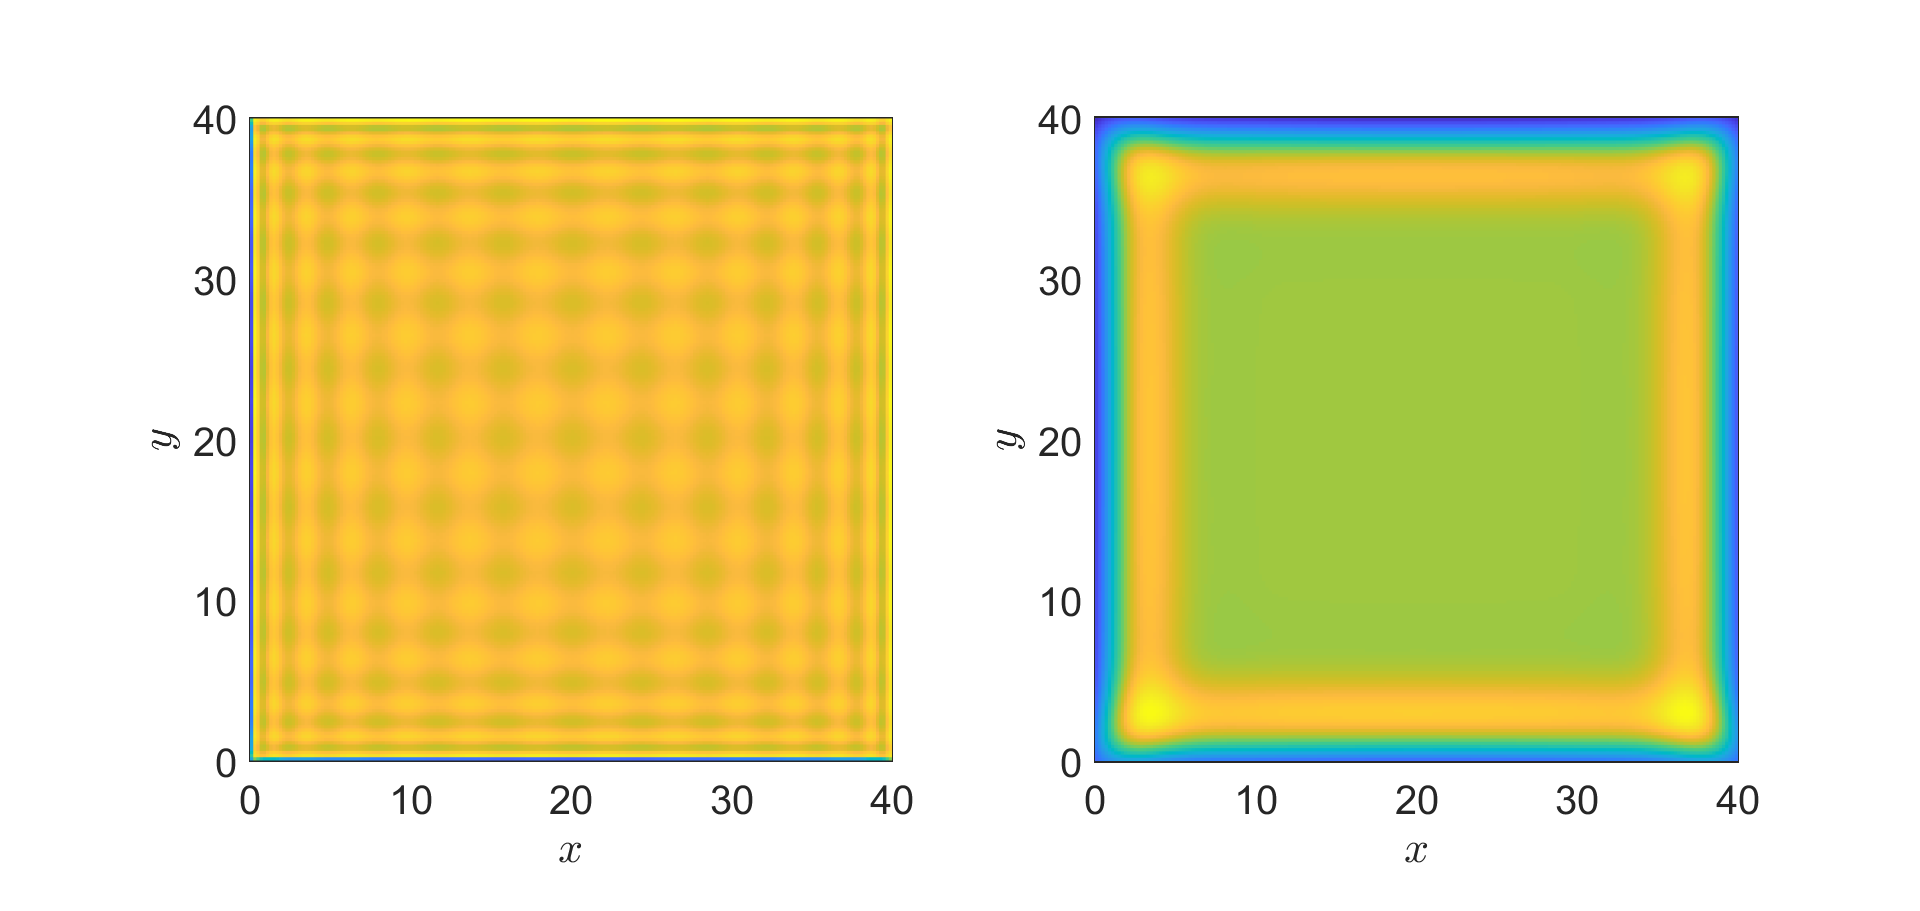
\includegraphics[scale=0.25]{OneShape3.png}
	\caption{Plot1 shows $V_{ext}$only, Plot2 shows $V_2$ only and Plot3 shows both. At time 1 and time 10 out of 20.} 
	\label{F10}
\end{figure}








\end{document}